\documentclass[11pt]{article}
\usepackage{geometry}
\geometry{letterpaper}

\usepackage{graphicx}
\usepackage{amssymb}
\usepackage{float}
\usepackage{tabularx}
\usepackage{multicol}
\usepackage{rotating}
\usepackage{hyperref}
\hypersetup{
    colorlinks,
    citecolor=black,
    filecolor=blue,
    linkcolor=black,
    urlcolor=black
}


% TODOs:
% ask Nick about lines in Seq Diagram, ask Nick about need 3D model, ask Nick about entering project goals
% switch to cleveref

\begin{document}

\begin{titlepage}
	\newcommand{\HRule}{\rule{\linewidth}{0.2mm}}
	\begin{center}
	\textsc{\LARGE McMaster University}\\[1.5cm]

	\textsc{\Large SmartServe}\\[0.5cm]
	\textsc{\large Software \& Mechatronics Capstone}\\[0.5cm]

	\HRule\\[0.4cm]
		{\huge\bfseries High Level System Design}\\[0.4cm]
	\HRule\\[0.4cm]

	\begin{minipage}[t][][t]{0.5\textwidth}
		\begin{flushleft} \large
			\emph{Authors:}\\
			Christopher McDonald - \textit{001312456} \\
			Harit Patel - \textit{001317372}\\
			Janak Patel - \textit{001307060} \\
			Jared Rayner - \textit{001311702}\\
			Nisarg Patel - \textit{001322805} \\
			Sam Hamel - \textit{001321692} \\
			Sharon Platkin - \textit{001316625} \\
		\end{flushleft}
	\end{minipage}
	~
	\begin{minipage}[t][][t]{0.4\textwidth}
		\begin{flushright} \large
			\emph{Professor:} \\
			Dr. Alan Wassyng \\[0.4cm]
			\emph{Teaching Assistants:} \\
			Bennett Mackenzie \\
			Nicholas Annable \\
			Stephen Wynn-Williams \\
			Viktor Smirnov
		\end{flushright}
	\end{minipage}\\[2cm]

	
\includegraphics[width=0.3\textwidth]{logo.png} \\
	{\large Last compiled on \today}
	\end{center}

\end{titlepage}

\tableofcontents
\listoffigures

\vfill
\begin{figure}[H]
   \centering
   \noindent\begin{tabularx}{\textwidth}{| >{\centering\arraybackslash}m{0.2\textwidth} | >{\centering\arraybackslash}m{0.2\textwidth} | >{\centering\arraybackslash}m{0.2\textwidth} | >{\centering\arraybackslash}m{0.285\textwidth} |}
   \hline
   \textbf{Date} & \textbf{Revision} & \textbf{Comments} & \textbf{Author(s)} \\ \hline
   Dec 1, 2017 & 1.0 & Main content done for all sections & Christopher McDonald \\ \hline
   Dec 13, 2017 & 1.1 & Corrected Document Overview & Nisarg Patel \\ \hline
   Dec 14, 2017 & 1.2 & Refined Project Scope \& System Description (Section 2) & Nisarg Patel \\ \hline
   Dec 17, 2017 & 1.3 & Added CRC card intro and reviewed & Christopher McDonald \\ \hline
   Dec 21, 2017 & 1.4 & Edited entire document & Sharon Platkin \\ \hline
   Dec 21, 2017 & 1.5 & Added Arduino Diagrams and Shooter Information & Nisarg Patel \\ \hline	
   Mar 9, 2018 & 2.0 & Added Likely / Unlikely Changes and Assumptions, Removed Shot Optimizer & Christopher McDonald \\ \hline	
   Mar 9, 2018 & 2.1 & Added motor specifications & Janak Patel \\ \hline	
   Mar 10, 2018 & 2.2 & Added details on CV and SR, fixed Start Sequence Diagram & Christopher McDonald \\ \hline
   Mar 10, 2018 & 2.3 & Fixed CRC cards for changes to requirements & Christopher McDonald \\ \hline
   Mar 18, 2018 & 2.4 & Converted to overall design, added in low level / component details & Christopher McDonald \\ \hline
   \end{tabularx}
   \caption{Revision History}
\end{figure}
\newpage
\section{Introduction}
\subsection{Project Overview}
SmartServe is an autonomous table tennis training system for table tennis players with various skill levels. SmartServe aids in diagnosing and improving a player's performance over time. The system trains table tennis players by shooting table tennis balls towards the player and detects successful returns from the player. The system can further adapt to the player's weaknesses and help them overcome it through further training. Importantly, SmartServe alleviates the problems of finding and working with a coach for players, as well as coaches trying to train multiple players simultaneously. The system will be deemed a success if the table tennis players and coaches can enjoy and see some value added by using SmartServe.\\\\
The project started at the beginning of the Fall 2017 academic term and will conclude at the end of the Winter 2018 term. In addition, the core project team consists of final year Software and Mechatronics Engineering students who are enrolled in the MECHTRON 4TB6/SFWRENG 4G06 capstone project course.
\subsection{Document Overview}
The purpose of this document is to provide an overview of the system design which meets the system requirements as specified in the \href{run:../Requirements/Requirements.pdf}{Requirements Document}. The system will be decomposed into subsystems, where each has responsibilities and is designed to fulfill certain requirements. The subsystems will have their intended input, expected output and description of how the module will be used. In further documentation, each will be designed in a way which is abstracted from this document's perspective. The expected use cases will also be detailed to understand the expectations of the user and how each subsystem interacts with one another. A more detailed view of this including timing as a factor will be detailed in the Sequence Diagram section. \\ \\ % TODO LINK EVERYTHING
For each subsystem, its purpose will be defined with respect to the overall system. After doing so, detailed input and output parameters will be defined. How each subsystem is architected is out of scope for this document and will be defined in further documentation. \\ \\

\subsection{Naming Conventions and Terminology}
\label{sec:definitions}
The following terms and definitions will be used throughout this document:
\begin{itemize}
% Alphabetical order is highly preferred as it eases user navigation
\item \textbf{ACID}: a database transaction which is atomic, consistent, isolated and durable
\item \textbf{CV}: computer vision
\item \textbf{FPS}: frames per second
\item \textbf{FSM}: finite state machine, shows transitions between states
\item \textbf{GUI}: graphical user interface
\item \textbf{IPO}: input process output
\item \textbf{Pitch}: rotation along the y-axis; this rotation angle primarily dictates the range of the ball from the net to the edge of the table on the user side
\item \textbf{Roll}: rotation along the x-axis
\item \textbf{Shooting Mechanism}: refers to the part of the system that shoots the table tennis balls towards the user side (player) Please refer to Figure \ref{fig:table-tennis-top-view} for visual illustration
\item \textbf{System}: encompasses both the hardware and software parts of SmartServe
\item \textbf{System Side}: the side of the table where the electromechanical system is placed; it is the opposite side of the User Side Please refer to Figure \ref{fig:table-tennis-top-view} for visual illustration
\item \textbf{TCP:} transmission control protocol
\item \textbf{Team}: all team members of the core capstone project, as noted in the list of Authors
\item \textbf{User Side}: the side of the table where the user (player) is standing
\item \textbf{Yaw}: rotation along the z-axis; this rotation angle primarily dictates the panning functionality of the shooting mechanism from the right side to the left side of the table
\end{itemize}

\begin{figure}[H]
   \centering
   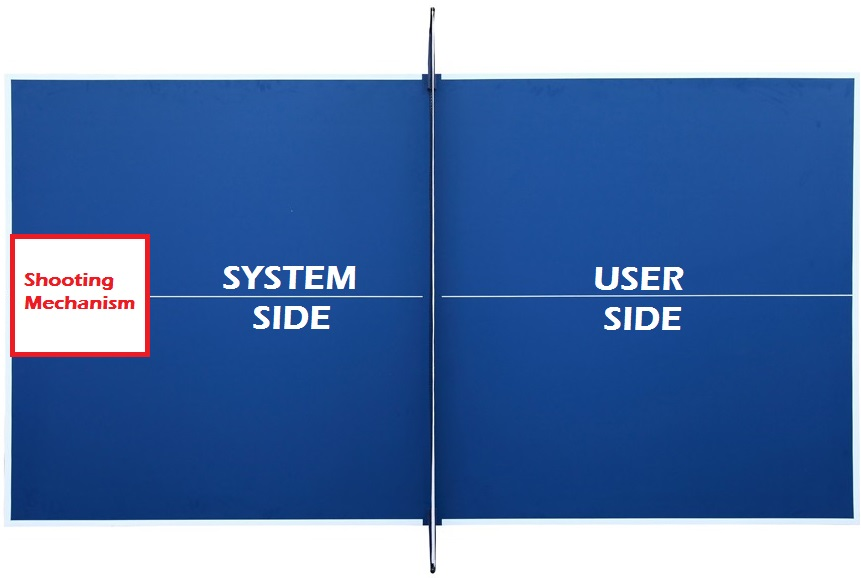
\includegraphics[width=0.75\textwidth]{img/Table-Tennis-Top-View.png} %requires the graphicx package
   \caption{Top View of the Tennis Table}
   \label{fig:table-tennis-top-view}
\end{figure}
\subsection{Project Scope}
The system will only attempt to shoot balls from the shooting mechanism straight towards the user side. Notably, the system will not attempt to return any shots from the user. After the user has returned a shot, the Computer Vision (CV) subsystem will be utilized to determine if the user's shot lands on the table or not. Additionally, the characteristics of the shot following any return will be determined by the system's mode and the proficiency of the player if available.
\subsection{Assumptions}
This design assumes the user supplies a functioning webcam, a capable computer to run the software and can connect to the SmartServe system via USB. The computer should have proficient computing power, as the CV subsystem will suffer in proficiency as a result. It is also assumed the use cases described here cover all interactions the user will attempt to have with the system. We assume the user has a ITTF-approved table, an orange table tennis ball and a paddle to use.
\section{System Description}
\subsection{System Architecture}
The system will follow a service-oriented architecture. This means that a central subsystem will interface with several services that serve a single purpose. Some subsystems will be simply told what needs to be done and others will be asked for some return value. This is done to implement separation of concerns where one subsystem doesn't know everything about the system and only what is necessary to satisfy their requirements. It also allows for easy increments of versioning, where one subsystem can be used as long as it is functional and easily swapped out for a newer version with extra features or increased performance. Moreover, this system has heavy timing constraints and an unpredictable environment so some actions must be taken in absence of a service's response. For example, the computer vision may take longer to track a ball depending on its trajectory where the system must shoot another ball in order to keep the user engaged.

\subsection{Subsystems}
The system will be broken down into subsystems with the following purposes: 
\begin{itemize}
\item \textbf{SmartServe}: general management of subsystems
\item \textbf{Computer Vision}:  detection of returns
\item \textbf{Shooting Mechanism}:  shooting the ball toward the user
\item \textbf{Shot Recommendation}: provides best shot
\item \textbf{Data Storage}: storing the data
\item \textbf{Shooting Model}: modelling the shot's trajectory
\item \textbf{User Interface}: taking input from the user and showing output
\end{itemize}
The diagram for this breakdown can be found in Figure \ref{fig:sub}.
\begin{figure}[H]
   \centering
   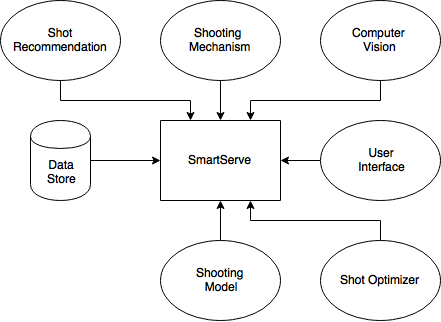
\includegraphics[width=0.6\textwidth]{img/Subsystem.png} % requires the graphicx package
   \caption{Subsystem Breakdown}
   \label{fig:sub}
\end{figure}
\subsection{Use Cases}
The diagram including all use cases can be found in Figure \ref{fig:usecase}. The user-instantiated ones will be described in detail below.
\begin{figure}[H]
   \centering
   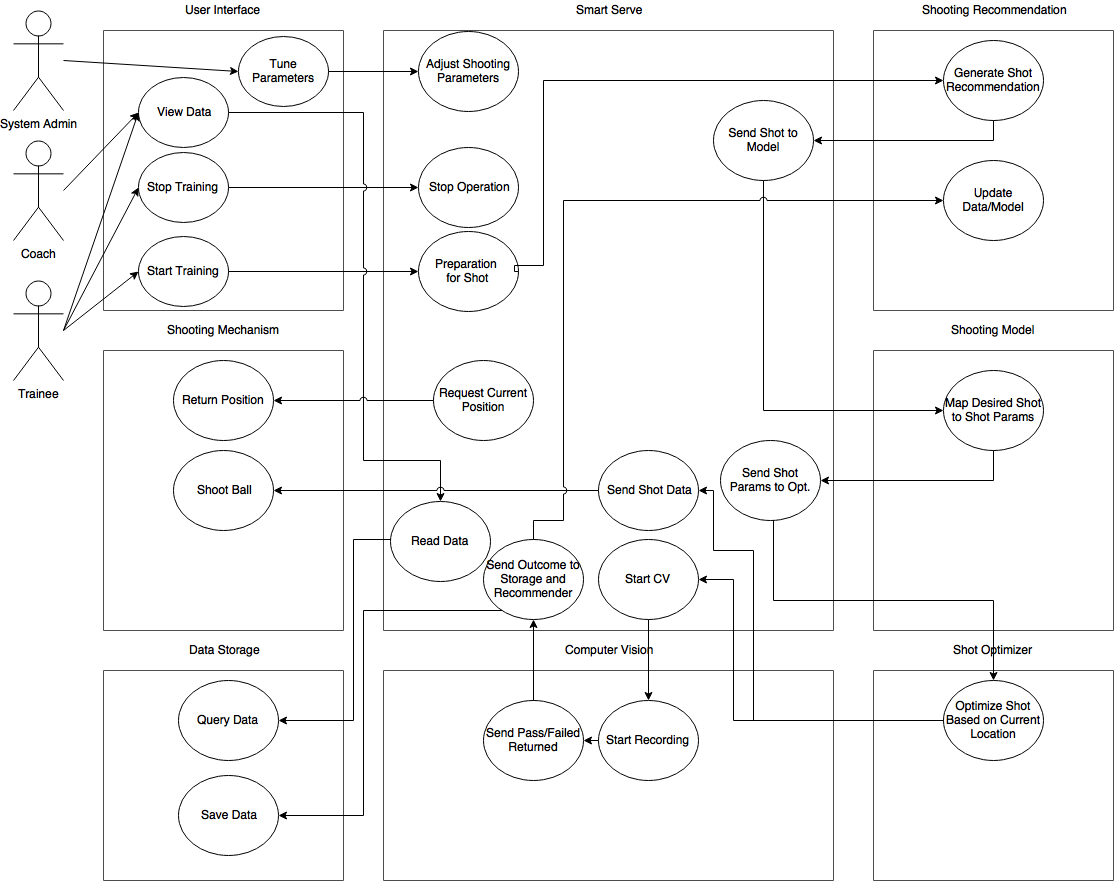
\includegraphics[width=\textwidth]{img/UseCase.png} % requires the graphicx package
   \caption{Use Case Diagram}
   \label{fig:usecase}
\end{figure}
\subsubsection{Start Training}
The user interface will have ways to allow the user to start this action which makes the Smart Serve subsystem prepare for a shot to shoot towards the user. To do this, it needs to request a shot to use from the Shot Recommendation subsystem. The shot includes the following parameters: desired location on the table, the speed of the shot and the angular velocity of the ball. The Smart Serve subsystem can then use the Shooting Model to translate this information into pitch, yaw and angular velocity to shoot the ball so it matches the desired shot. After doing so, it will instruct the shooting mechanism to shoot the ball with the appropriate parameters and start the CV subsystem to begin tracking for a successful return. Only until the CV subsystem returns the pass or failed return data, can it update the Data Storage and Shot Recommendation subsystems with this new information. The former will store the result and the data for the shot together, where the latter will update the model used to generate shot recommendations. Upon completion, it can begin preparing for a new shot.
\begin{figure}[H]
   \centering
   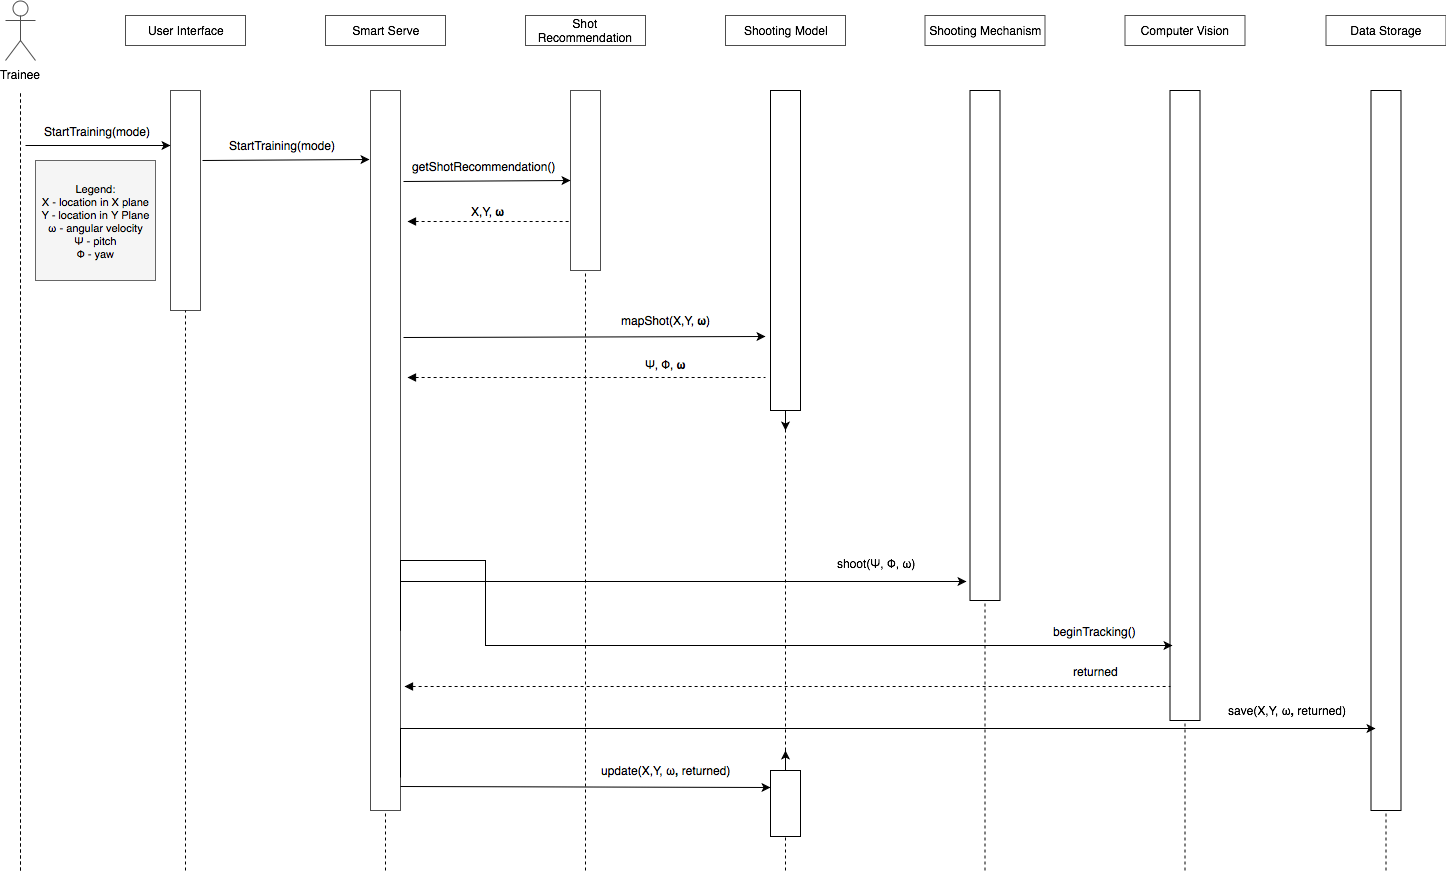
\includegraphics[width=\textwidth]{img/SequenceDiagram-Start.png}
   \caption{Sequence Diagram for Starting Training}
   \label{fig:start}
\end{figure}
\subsubsection{Stop Training}
In the event the user wants to cease training, the user interface will allow this and will halt the system from shooting balls. No data should be written nor shots requested for the shooting mechanism to shoot in order to preserve the integrity of the data being gathered.
\begin{figure}[H]
   \centering
   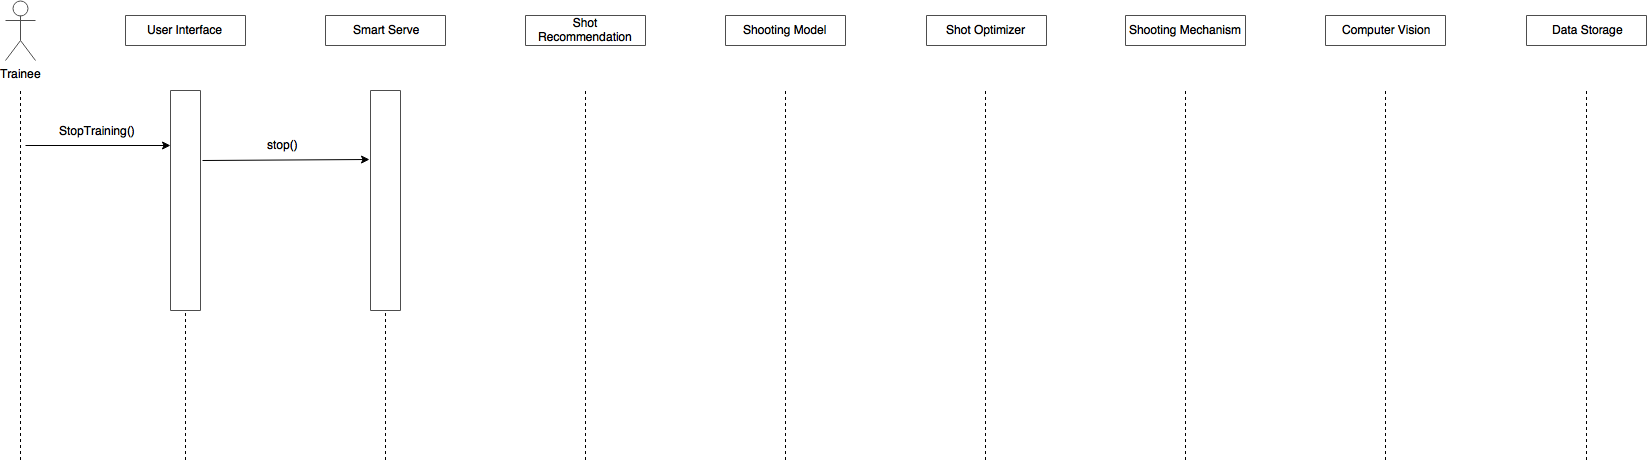
\includegraphics[width=\textwidth]{img/SequenceDiagram-Stop.png}
   \caption{Sequence Diagram for Ceasing Training}
   \label{fig:stop}
\end{figure}
\subsubsection{View Results}
When the user wants to visualize the results of their performance, the user interface should be used. It will use the Smart Serve subsystem to query data from Data Storage and present it in some meaningful way.
\begin{figure}[H]
   \centering
   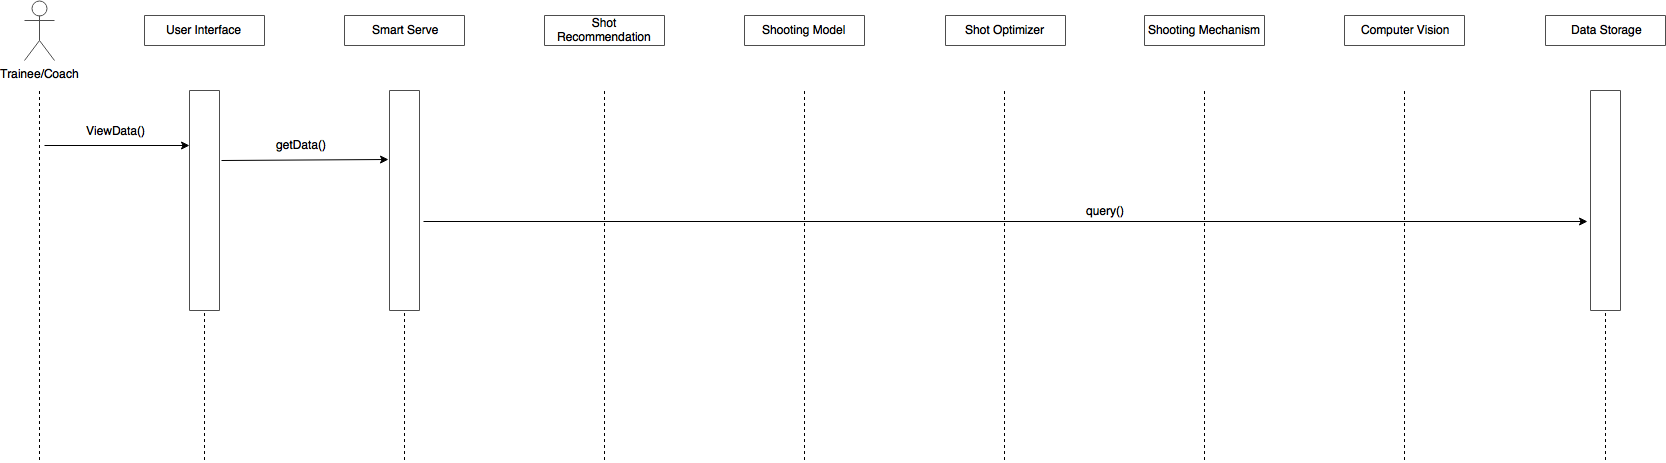
\includegraphics[width=\textwidth]{img/SequenceDiagram-View.png}
   \caption{Sequence Diagram for Viewing Training Results}
   \label{fig:view}
\end{figure}
\subsubsection{Tune Parameters}
The system may need to be adjusted for various lighting, table sizes or environments. The user interface will allow a system administrator to do this in order to directly change values associated for these variables.
\begin{figure}[H]
   \centering
   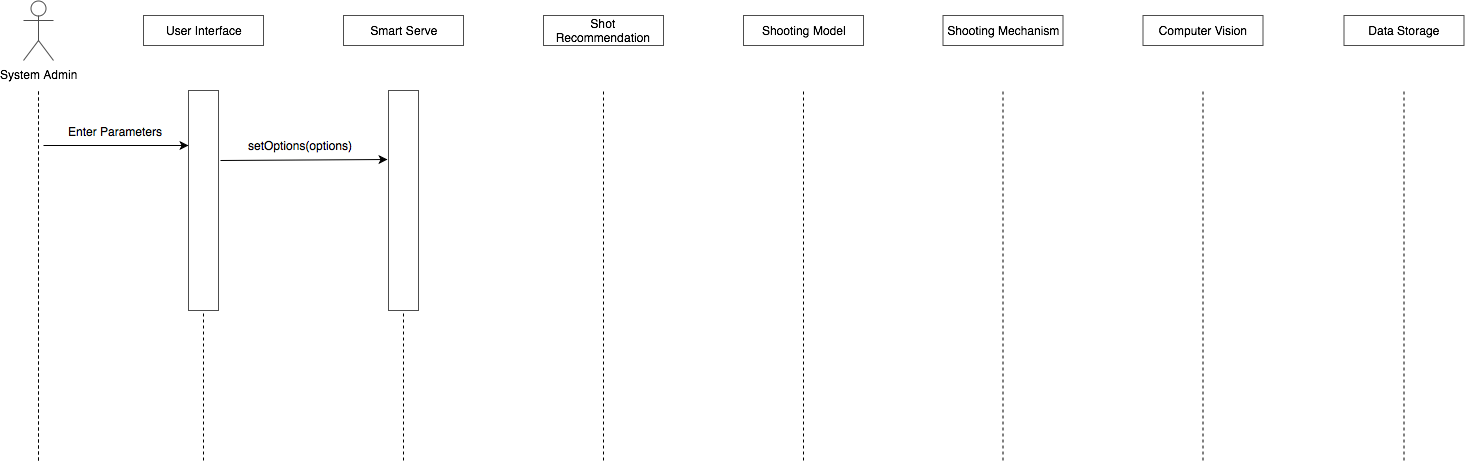
\includegraphics[width=\textwidth]{img/SequenceDiagram-Tune.png}
   \caption{Sequence Diagram for Tuning Parameters}
   \label{fig:tune}
\end{figure}
\subsubsection{Start System}
The user interface will allow the system to be booted which will start the Smart Serve subsystem. This will allow the Shot Recommendation system to build its model based on previous data for the user, if it exists.
\begin{figure}[H]
   \centering
   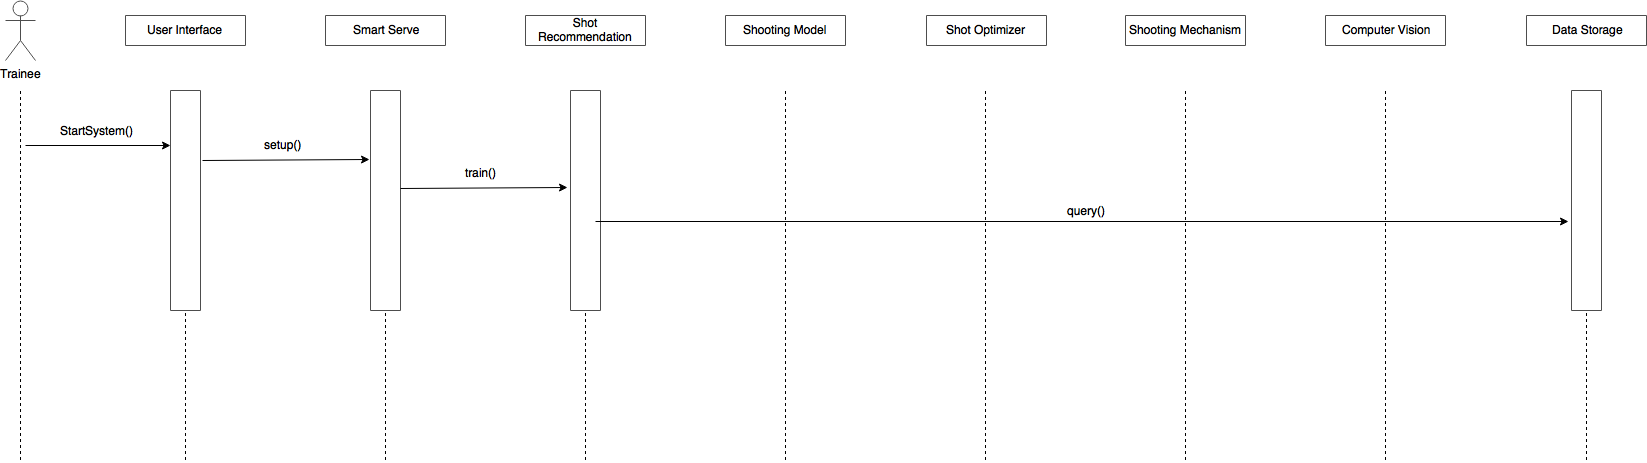
\includegraphics[width=\textwidth]{img/SequenceDiagram-Boot.png}
   \caption{Sequence Diagram for Booting the System}
   \label{fig:boot}
\end{figure}

\subsection{Behaviour Description}
As the behaviour of the system has been discussed previously, this section will describe the expected user behaviour and how they will interact with the system.
\subsubsection{Normal Operation}
The trainee would begin by starting the system from its off state. This will trigger the Start System use case. The user will then trigger the Start Training use case and specify a training mode. This creates the loop of Smart Serve prepping and serving shots for the user. Only until the user triggers the Stop System use case will this loop stop during normal operation. During or after training a user can start the View Data use case to get details on their performance.
\subsubsection{Abnormal Operation}
Although possible, there are some actions a user could take which would be considered abnormal. If a user hits the ball and it immediately leaves the viewable area of the computer vision, whether it never returns or does so after 1.5 seconds, it should be considered a failed return. A user could also replace the table with a different one without calibrating the system to the new table. Furthermore, the user could misplace the system such that it is not centre with the table or at the edge of the table. The proper placement can be found in Figure \ref{fig:table-tennis-top-view}. The system will require the user to load the balls into the shooting mechanism's hopper which will need to be a particular size and colour to work optimally.
\subsubsection{Error Handling}
If the system should encounter an error, it should display the details of it through the User Interface subsystem. In addition to this, it must take measures to ensure the safety of the user and integrity of the system. This includes stopping all training and pending actions for the system to perform. Examples of such errors include a jammed table tennis ball, and an empty mechanism ball hopper.
\subsection{Likely Changes}
Some aspects of the system design will likely change as the project progresses which will be excluded within this document. This is done so the design is considered complete and the next stages of design and implementation can be done. The first likely change would be to the computer vision subsystem, as the introduction of another camera would change the high level design of this subsystem. The additional camera would track a 3rd dimension, which is along the short side of the table. This change would propagate through the system since the Shot Recommendation subsystem would need to consider this new data for recommending new shots. The Data Storage subsystem will also be changed to hold the new data.
\subsection{Unlikely Changes}
The overall architecture of the system will not change, although additional subsystems could be added or existing ones could be changed. The degrees of freedom for a shot will not change. The Smart Serve subsystem will likely not change, although the data being processed between states may change. 
\section{Subsystems Overview}
\subsection{Smart Serve}
The Smart Serve subsystem will provide the means of interfacing with all the subsystems and enforcing timing constraints. For all intents and purposes, it can be considered the main process and hub of the system. In the event a subsystem is taking too long to respond, this subsystem must be able to continue operation to meet timing requirements. The various states and transitions can be found in Figure \ref{fig:fsm}. The FSM (Finite State Machine) diagram shows each state should have an \textit{exit option} if a service takes longer than allowed to preform an action.
\begin{figure}[H]
   \centering
   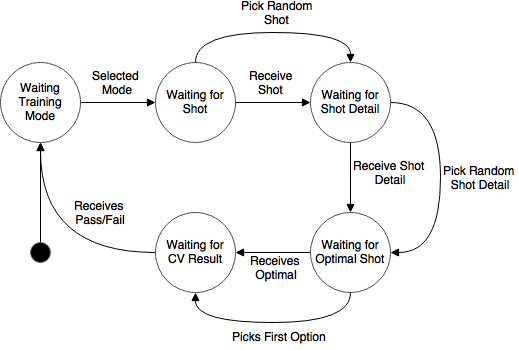
\includegraphics[width=0.7\textwidth]{img/FSM.png}
   \caption{Smart Serve FSM}
   \label{fig:fsm}
\end{figure}

\subsection{Computer Vision}
The Computer Vision subsystem will be a service to the Smart Serve subsystem to determine if a shot is successfully returned. When sent a request to begin tracking the ball, it will do so and return a true when the ball bounces off the table or false when it doesn't. In the event the ball never enters frame, it will assume the return was failed after a fixed amount of time. \\ \\
The FSM will be updated every frame captured within the CV subsystem. Once a frame is captured, the position of the ball will be compared against the previous position and a difference in position can be calculated. Based on how it moved, the state of the FSM will or will not change. Since the ball is being viewed on the System's side, a valid return is when it is moving towards the system, travels downward and then upward while still in frame. The states and transitions of the FSM represent this.
\begin{figure}[H]
   \centering
   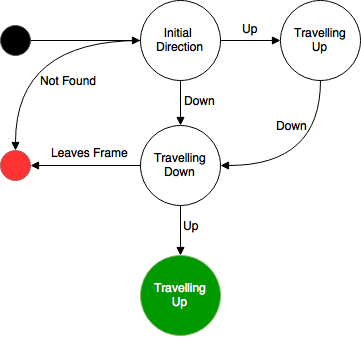
\includegraphics[width=0.4\textwidth]{img/cvFSM.png}
   \caption{CV Finite State Machine}
   \label{fig:cv}
\end{figure}
\subsection{Shot Recommendation}
The Shot Recommendation subsystem will be a service to the Smart Serve subsystem to determine which shot should be taken next. The way the subsystem decides on the shot will be determined by the training mode the user selects. These will include shooting the same shot every time, pseudo-randomly picking a shot or using reinforcement learning algorithms to decide the next shot. The last mode will be based on previous performance by the user. \\ \\
The training mode will utilize a variation of a Upper Confidence Bound (UCB) algorithm. The subsystem will attempt to predict the actual return rate for each type of shot for a particular player by holding a range of values the actual return rate exists within. The initial state is from 0 - 100\% and the range for a individual shot closes when the shot is attempted. The minimum will rise if it is returned successfully and the maximum is lowered if the player misses it. When a shot is needed, the subsystem will select one shot from the shots with the lowest minimum bound since they have the highest chance of being the player's weakest points. This provides the important benefit of exploring different shots at the beginning and exploiting some later in the training phase. 
\subsection{Shooting Model}
The Shooting Model subsystem will be a service to the Smart Serve subsystem which provides the means of mapping a desired shot to the details needed to take the shot. The input and output for the system can be found in Figure \ref{fig:shotmodel}. The output will be an array of many combinations of pitch, yaw, speed and angular velocity that satisfy the input shot details.
\begin{figure}[htbp]
   \centering
   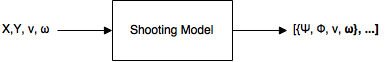
\includegraphics[width=0.6\textwidth]{img/ShotModel.png} % requires the graphicx package
   \caption{Shooting Model I/O}
   \label{fig:shotmodel}
\end{figure}
\subsection{Data Storage}
The Data Storage subsystem will store all the details for each shot, the user's profile and the return rates for each user. It will need to have interfaces for saving data and querying data out of the system in a variety of formats. Ideally, it will require minimal detail and configuration for the subsystem which uses it due to the variety of implementations of these subsystems.
\subsection{User Interface}
The User Interface subsystem will be the means of translating user requests into actionable requests for the Smart Serve subsystem. The inputs will include a username, password, mode selection and some means of starting and stopping the training. The UI will also need to accept custom parameters for performance data including time ranges and ways to cluster shot types. The output will include custom and useful error messages as well as graphs and tables for performance data.
\subsection{Shooting Mechanism}
The Shooting Mechanism will be the subsystem which fires the ball towards the user. A microcontroller will be used as the point of contact and set any actuators required to fire a specified shot. It must complete this action within 1.5 seconds for the Computer Vision to detect the ball returned by the user. \\\\
The Shooting Mechanism will consist of three main sub parts: Automatic Feeder, Automatic Panning, Ball Shooter. The functionality of the Automatic Feeder part will be to automatically control the feeding rate of the table tennis balls into the shooting barrel and feed the balls into the barrel as initiated by the program. The functionality of the Automatic Panning will be to rotate the entire shooting mechanism or the shooting barrel about the z-axis so the mechanism is able to cover all of the shooting zones as specified in the requirements. Additionally, the functionality of the ball shooter is actually shoot out table tennis balls from the shooting barrel. Please refer to figure \ref{fig:shootingmechanismoutline} for visual representation. \\\\
In terms of electrical components, Arduino UNO microcontroller will be used to control all of the IPO (Input Process Output) processes between the sensors, actuators and Smart Serve. For the ball shooter, a DC Motor will be used as the system will require high speeds and high torques to shoot out table tennis balls. The details on the DC motor can be found below in Table \ref{table:motorspecs} (SAYAL Electronics SKU No. 230437). The DC Motor will be controlled using the PWM method for speed control. Additionally, a Stepper Motor will be utilized for the automatic feeding of the balls into shooting barrel functionality as the Stepper motor would not require any position encoder as well as the stepper motor will have predictable movements. Details on the stepper motor can be found below in Table \ref{table:feedermotorspecs} (Grobotronics SKU No. 19-00012858). For the automatic panning part of the shooting mechanism, a servo or a stepper motor will be utilized however that would be further refined after rigorous prototyping and simulations. Please refer to Figure \ref{fig:electricalwiringdiagrambb}, Figure \ref{fig:electricalwiringdiagramschematic}, and Figure \ref{fig:electricalwiringdiagrampcb} for an overview of Electrical Bread Board, Schematic and PCB layout diagrams of how the Shooting Mechanism system outline.

\begin{table}[H]
\begin{center}
\begin{tabular}{|c|c|}
	\hline 
	Motor Type & DC \\ 
	\hline 
	Operating Voltage & 3V - 6V DC \\ 
	\hline 
	Max. Speed & 17000 rpm \\ 
	\hline 
	Shaft Diameter & 2 mm \\ 
	\hline 
	Torque & 20.72 g-cm \\ 
	\hline 
\end{tabular} 
\caption{Shooting Motor Specifications}
\label{table:motorspecs}
\end{center}

\begin{center}
	\begin{tabular}{|c|c|}
		\hline 
		Motor Type & Uni-polar Gear Stepper with Driver \\ 
		\hline 
		Operating Voltage & 5V DC \\ 
		\hline 
		Max. Speed & 80rpm over-driving with 9V \\ 
		\hline 
		Holding Torque & 350 g-cm \\ 
		\hline 
		Step Angle (output shaft) & 5.625$^{\circ}$/64 \\ 
		\hline 
		Gear Ratio & 1/64 reduction \\ 
		\hline 
		Steps per Rev. & 512 \\ 
		\hline 
		Shaft & Flattened for set-screw attachment \\ 
		\hline 
	\end{tabular} 
	\caption{Feeder Motor Specifications}
	\label{table:feedermotorspecs}
\end{center}
\end{table}



\begin{figure}[H]
   \centering
   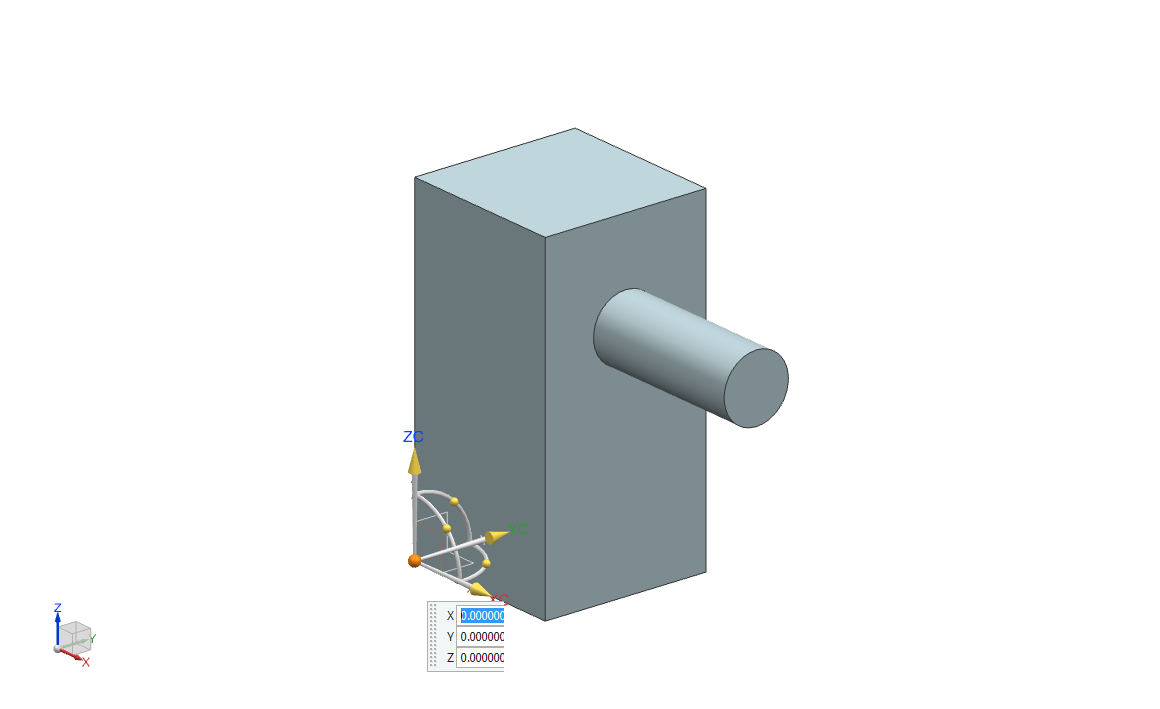
\includegraphics[width=1\textwidth]{img/Shooting_Mechanism.png} %requires the graphicx package
   \caption{Shooting Mechanism Rough Outline}
   \label{fig:shootingmechanismoutline}
\end{figure}

\begin{figure}[H]
   \centering
   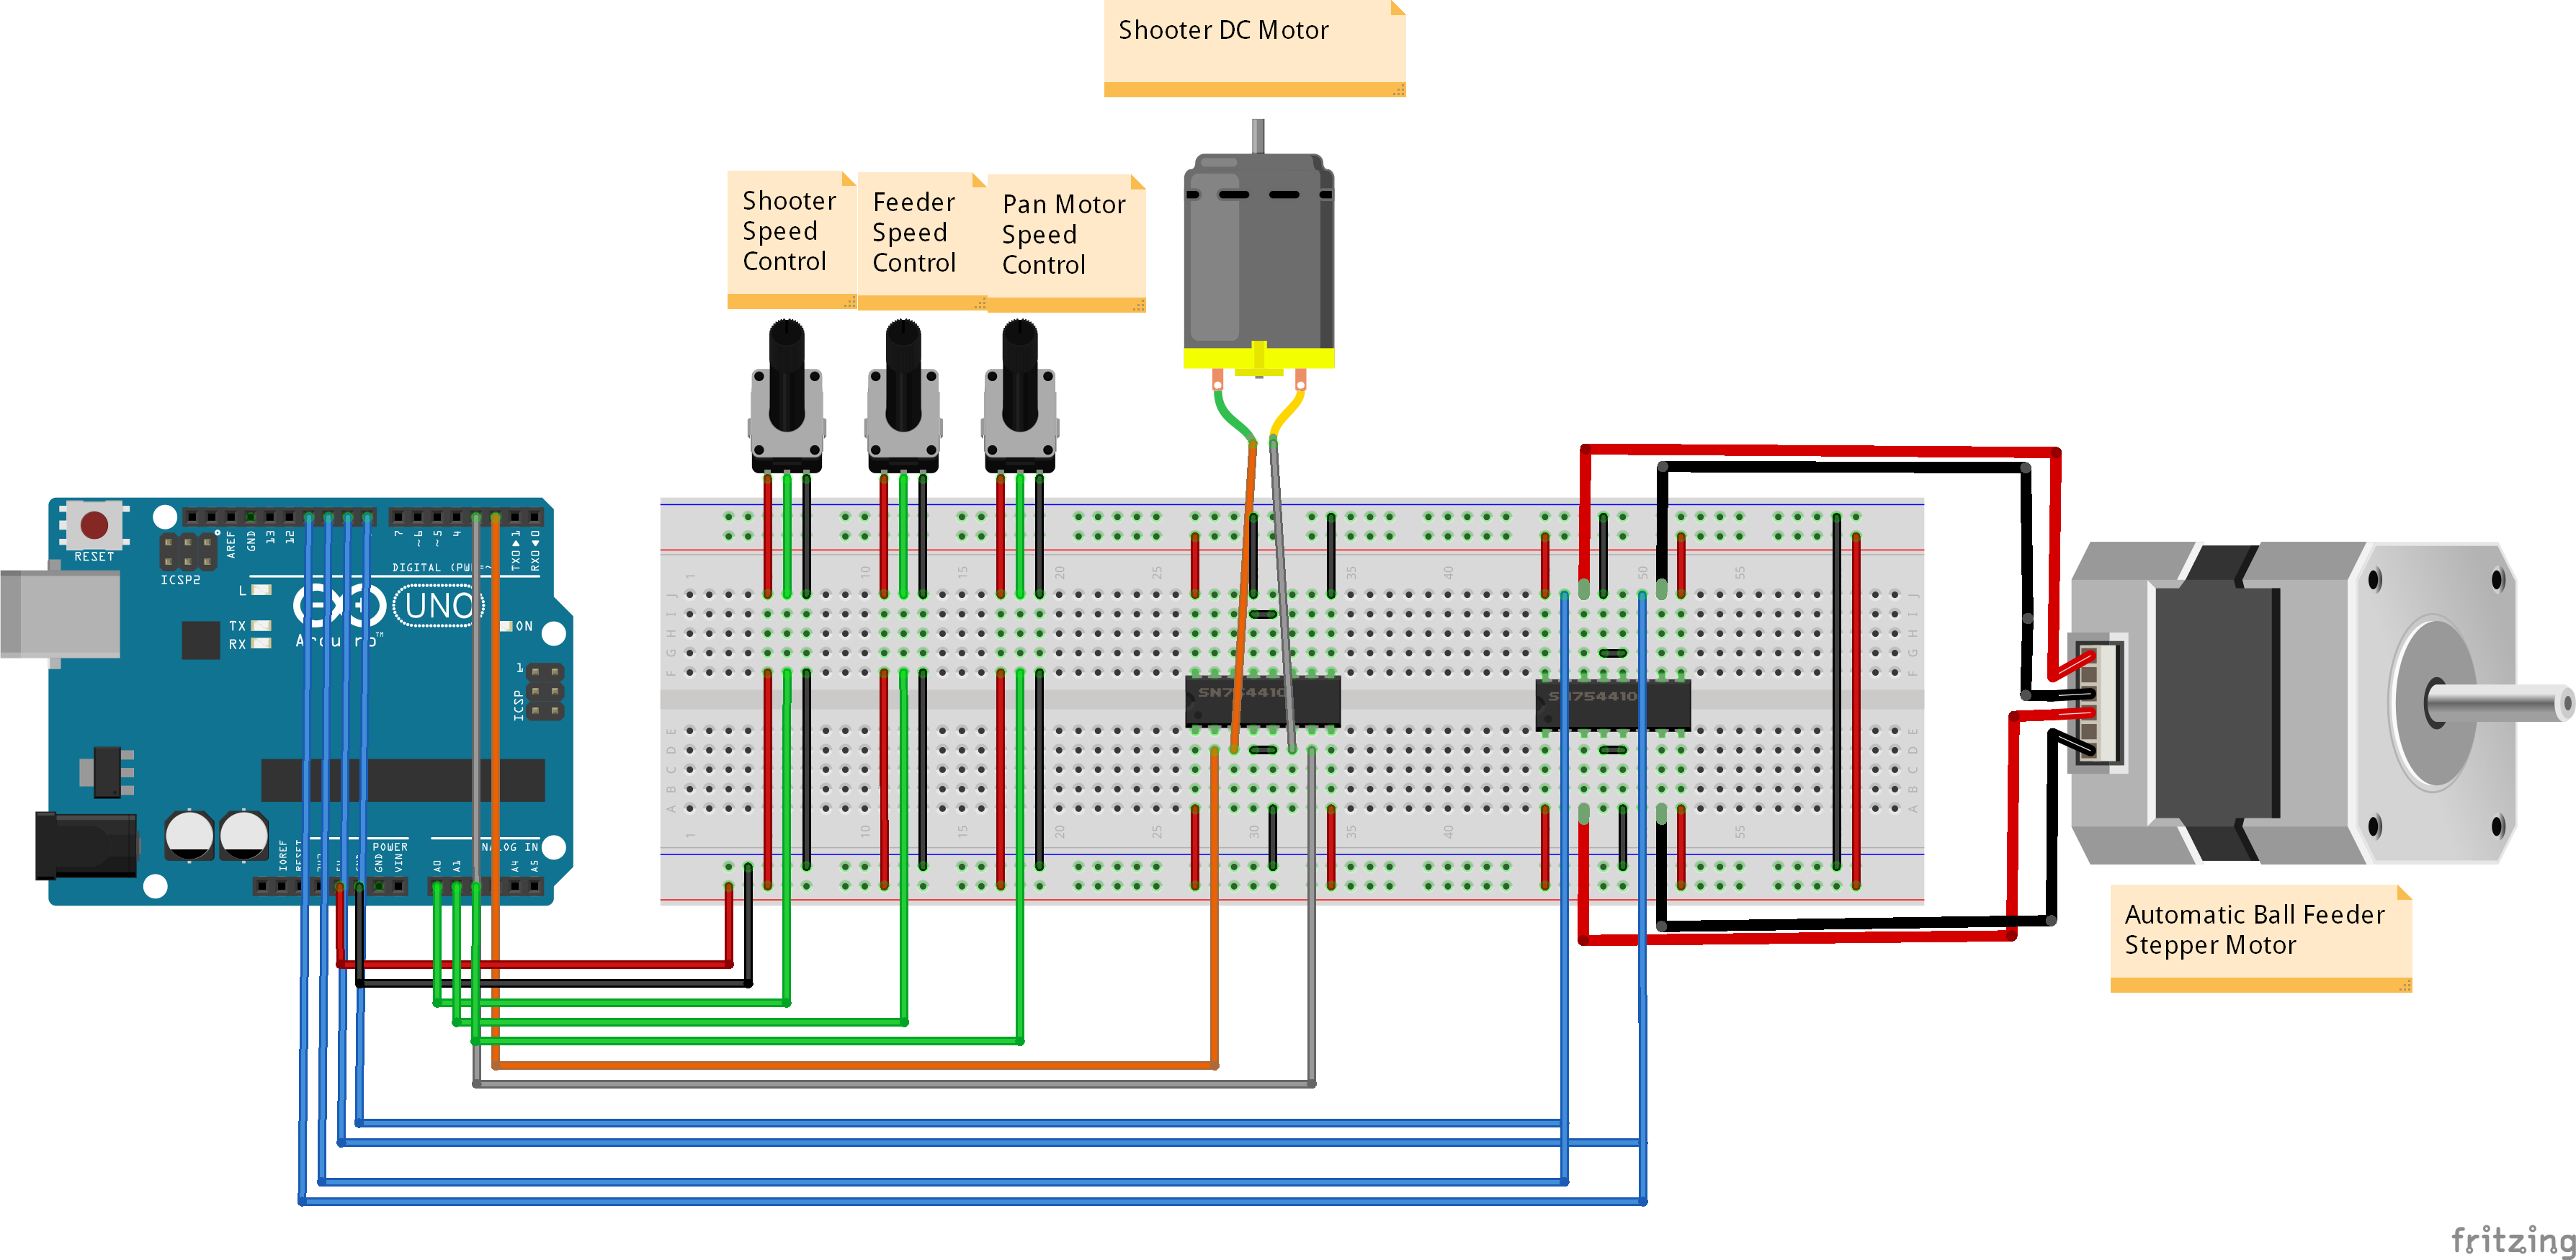
\includegraphics[width=1\textwidth]{img/Electrical_Wiring_Diagram_bb.png} %requires the graphicx package
   \caption{Electrical Wiring Diagram - Bread Board}
   \label{fig:electricalwiringdiagrambb}
\end{figure}

\begin{figure}[H]
   \centering
   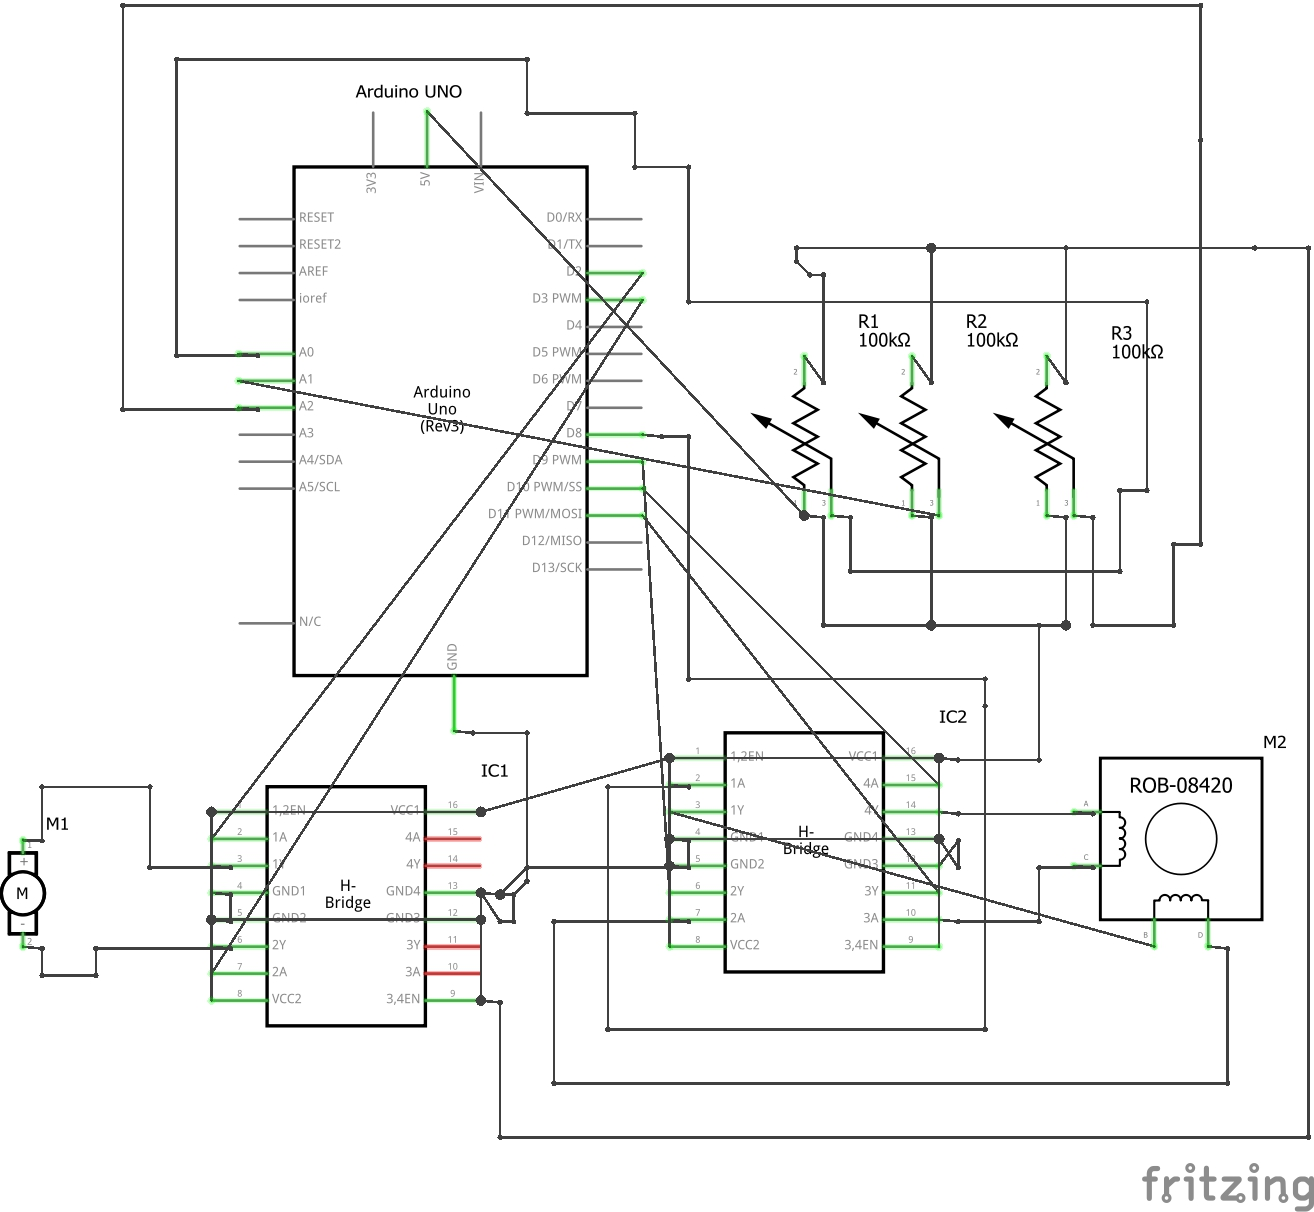
\includegraphics[width=1\textwidth]{img/Electrical_Wiring_Diagram_schematic.png} %requires the graphicx package
   \caption{Electrical Wiring Diagram - Schematic}
   \label{fig:electricalwiringdiagramschematic}
\end{figure}

\begin{figure}[H]
   \centering
   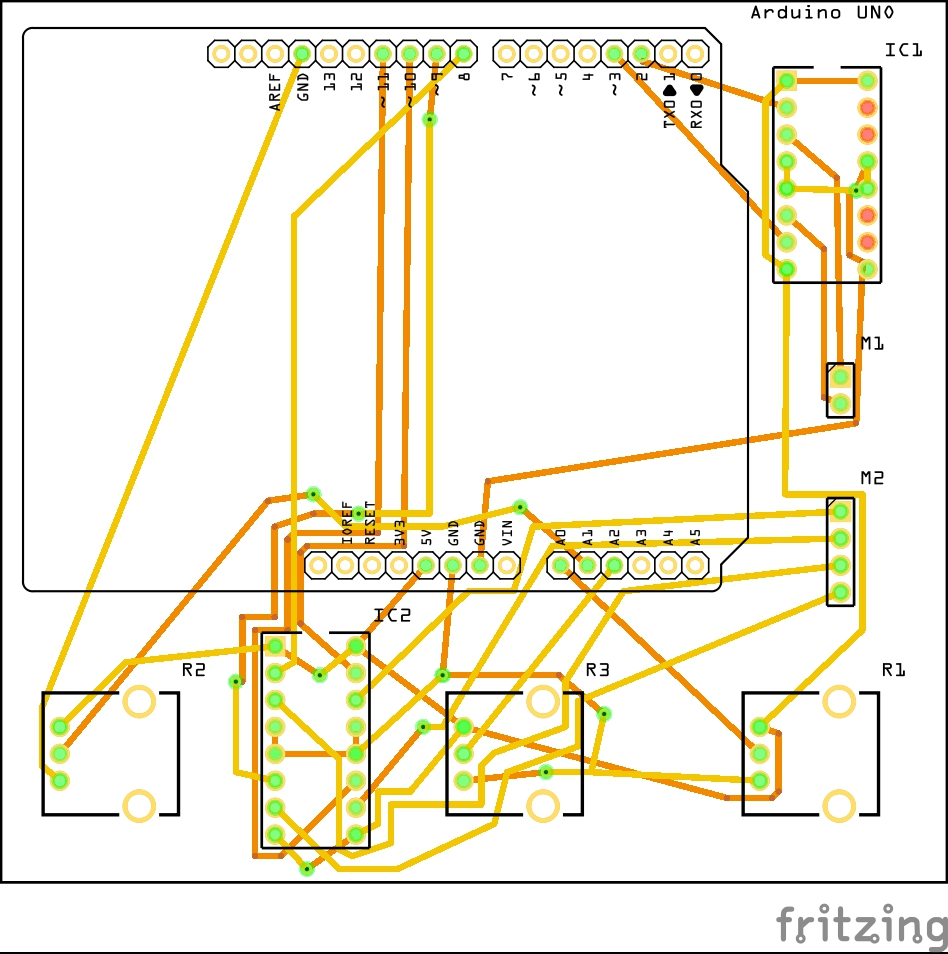
\includegraphics[width=1\textwidth]{img/Electrical_Wiring_Diagram_pcb.png} %requires the graphicx package
   \caption{Electrical Wiring Diagram - Printer Circuit Board Trace}
   \label{fig:electricalwiringdiagrampcb}
\end{figure}



\section{Class Responsibility Collaboration (CRC) Cards}
The following sections will include one CRC card for each subsystem. A CRC card contains information pertaining to which requirements a subsystem is responsible for and which subsystems one would collaborate with. This will be used for testing purposes and to track where a given requirement is satisfied. A requirement does not have to be satisfied completely by one subsystem, but a majority of the work must be done by that subsystem.
\subsection{SmartServe}

\begin{table}[H]
\centering
\label{my-label}
\begin{tabular}{ | >{\raggedright\arraybackslash}p{0.4\textwidth} | >{\raggedright\arraybackslash}p{0.4\textwidth} | }
\hline
\multicolumn{2}{|c|}{\textbf{Smart Serve}}             \\ \hline
\textbf{Responsibilities:} & \textbf{Collaborators:} \\ \hline
\begin{itemize}
\item \textbf{F10}: pause the shooting mechanism
\item \textbf{F18}: shoot a ball once the previous has been returned to the system side or 1.5 seconds after the previous shot, whichever is shorter
\item \textbf{P2}:  must include all but previous 3 shots in performance data
\item \textbf{P5}: must support only one user playing at one time
\end{itemize}
&
\begin{itemize}
\item Computer Vision
\item Shot Recommendation
\item Shooting Model
\item Data Storage
\item User Interface
\item Shooting Mechanism
\end{itemize} \\ \hline
\end{tabular}
\caption{Smart Serve CRC Card}
\end{table}

\subsection{Computer Vision}

\begin{table}[H]
\centering
\label{my-label}
\begin{tabular}{ | >{\raggedright\arraybackslash}p{0.4\textwidth} | >{\raggedright\arraybackslash}p{0.4\textwidth} | }
\hline
\multicolumn{2}{|c|}{\textbf{Smart Serve}}             \\ \hline
\textbf{Responsibilities:} & \textbf{Collaborators:} \\ \hline
\begin{itemize}
\item \textbf{F5}: detect a successful return by the user
\item \textbf{OE2}: functional in indoor settings with bright florescent lighting
\end{itemize}
&
\begin{itemize} \item Smart Serve
\end{itemize} \\ \hline
\end{tabular}
\caption{Computer Vision CRC Card}
\end{table}

\subsection{Shot Recommendation}

\begin{table}[H]
\centering
\label{my-label}
\begin{tabular}{ | >{\raggedright\arraybackslash}p{0.4\textwidth} | >{\raggedright\arraybackslash}p{0.4\textwidth} | }
\hline
\multicolumn{2}{|c|}{\textbf{Smart Serve}}             \\ \hline
\textbf{Responsibilities:} & \textbf{Collaborators:} \\ \hline
\begin{itemize}
\item \textbf{F7}: load a previously saved state
\item \textbf{F14}: implements a training mode
\end{itemize}
&
\begin{itemize}
\item Smart Serve
\item Data Storage
\end{itemize} \\ \hline
\end{tabular}
\caption{Shot Recommendation CRC Card}
\end{table}

\subsection{Shooting Model}

\begin{table}[H]
\centering
\label{my-label}
\begin{tabular}{ | >{\raggedright\arraybackslash}p{0.4\textwidth} | >{\raggedright\arraybackslash}p{0.4\textwidth} | }
\hline
\multicolumn{2}{|c|}{\textbf{Smart Serve}}             \\ \hline
\textbf{Responsibilities:} & \textbf{Collaborators:} \\ \hline
\begin{itemize}
\item \textbf{F14}: implements a training mode
\item \textbf{F15}: implements a one-shot mode
\end{itemize}
&
\begin{itemize}
\item Smart Serve
\end{itemize} \\ \hline
\end{tabular}
\caption{Shooting Model CRC Card}
\end{table}

\subsection{Data Storage}

\begin{table}[H]
\centering
\label{my-label}
\begin{tabular}{ | >{\raggedright\arraybackslash}p{0.4\textwidth} | >{\raggedright\arraybackslash}p{0.4\textwidth} | }
\hline
\multicolumn{2}{|c|}{\textbf{Smart Serve}}             \\ \hline
\textbf{Responsibilities:} & \textbf{Collaborators:} \\ \hline
\begin{itemize}
\item \textbf{F6}: saves details for each shot taken by the shooting mechanism
\item \textbf{F8}: allows creation of a new user
\item \textbf{F9}: authenticate users
\item \textbf{P4}: must support 1000 users
\item \textbf{MS2}: able to add new metrics to analyze performance
\item \textbf{S1}: hash all passwords for user profiles
\item \textbf{S2}: encrypt all performance data for each user
\item \textbf{P1}: allow read access for coaches
\end{itemize}
&
\begin{itemize}
\item Shot Recommendation
\item Smart Serve
\end{itemize} \\ \hline
\end{tabular}
\caption{Data Storage CRC Card}
\end{table}

\subsection{User Interface}

\begin{table}[H]
\centering
\label{my-label}
\begin{tabular}{ | >{\raggedright\arraybackslash}p{0.4\textwidth} | >{\raggedright\arraybackslash}p{0.4\textwidth} | }
\hline
\multicolumn{2}{|c|}{\textbf{Smart Serve}}             \\ \hline
\textbf{Responsibilities:} & \textbf{Collaborators:} \\ \hline
\begin{itemize}
\item \textbf{F11}: end the training session
\item \textbf{F12}: resume training session from a paused state
\item \textbf{F13}: display user's performance over a custom time range
\item \textbf{F16}: allows user to adjust training parameters during an active or paused session
\item \textbf{F17}: can be calibrated for a specific table size
\item \textbf{LF1}: have a minimalist design that is easy to navigate through
\item \textbf{UH1}: is intuitive to use
\item \textbf{UH2}: operable using the English language
\item \textbf{P1}: response time for user input must be less than or equal to 100ms
\end{itemize}
&
\begin{itemize}
\item Smart Serve
\end{itemize} \\ \hline
\end{tabular}
\caption{User Interface CRC Card}
\end{table}

\subsection{Shooting Mechanism}

\begin{table}[H]
\centering
\label{my-label}
\begin{tabular}{ | >{\raggedright\arraybackslash}p{0.5\textwidth} | >{\raggedright\arraybackslash}p{0.5\textwidth} | }
\hline
\multicolumn{2}{|c|}{\textbf{Smart Serve}}             \\ \hline
\textbf{Responsibilities:} & \textbf{Collaborators:} \\ \hline
\begin{itemize}
\item \textbf{F1}: shoots the table tennis ball towards the user at various locations
\item \textbf{F2}: shoots the table tennis ball towards the user at various speeds
\item \textbf{F3}: shoots the table tennis ball towards the user at various degrees of Yaw
\item \textbf{F4}: shoots the table tennis ball towards the user with various degrees of roll
\item \textbf{HS1}: always hit the table at least once per shot
\item \textbf{HS2}: not shoot the ball faster than 22 m/s
\item \textbf{HS3}: have no exposed electrical wiring or components
\item \textbf{HS4}: carries warnings around moving parts
\item \textbf{HS5}: has a button to cease all power to system
\end{itemize}
&
\begin{itemize}
\item Smart Serve
\end{itemize} \\ \hline
\end{tabular}
\caption{Shooting Mechanism CRC Card}
\end{table}

\section{Detailed Class Diagram}
The Detailed Class Diagram is shown in Figure \ref{fig:dcd}, found in the Appendix.

\section{Module Guide}
\subsection{SmartServe Modules} % Chris - edited by Sharon
\subsubsection*{Controller}
\textbf{Responsibilities} \\
The controller handles all the timing constraints and sequential events for shooting balls towards the player. It is the interface for the UI to allow the user to preform any and all actions. \\ \\
\textbf{Secrets} \\
The sequence and timing constraints of the shooting procedure. \\ \\
\textbf{MID}
\begin{itemize}
\item \textbf{boot} - none \\ returns: \textit{boolean} \\ description: instantiates all dependancies and ensures services are working as expected
\item \textbf{startTraining} - Mode m \\ returns: \textit{boolean} \\ description: starts the shooting procedure given a certain training Mode
\item \textbf{stopTraining} - none \\ returns: \textit{boolean} \\ description: stops the training procedure
\item \textbf{setShootingParameters} - ShootingParameters sp \\ returns: \textit{boolean} \\ description: sets the shooting parameters for certain table sizes
\end{itemize}

\subsubsection*{ArduinoConnector}
\textbf{Responsibilities} \\
This module is responsible for facilitating the communication with the Arduino which is part of the Shooting Mechanism subsystem (SM). This includes sending and receiving messages as well as ensuring proper testing of the connection is preformed. \\ \\
\textbf{Secrets} \\
The connection to the Arduino. \\ \\
\textbf{MID}
\begin{itemize}
\item \textbf{test} - int port \\ returns: \textit{boolean} \\ description: tests connection to the Arduino
\item \textbf{shoot} - float pitch, float yaw, float angularVelocity \\ returns: \textit{none} \\ description: instructs Arduino to shoot the ball in a certain way
\item \textbf{position} - none \\ returns: \textit{Position} \\ description: returns the position of the mechanism
\end{itemize}

\subsubsection*{ShotRecommendationConnector}
\textbf{Responsibilities} \\
This module is responsible for facilitating the communication with the ShotRecommendation subsystem (SR). This includes sending and receiving messages as well as ensuring proper testing of the connection is preformed. \\ \\
\textbf{Secrets} \\
The connection to the SR. \\ \\
\textbf{MID}
\begin{itemize}
\item \textbf{connect} - int port, [optional] String ip \\ returns: \textit{boolean} \\ description: instantiates all dependancies and ensures services are working as expected
\item \textbf{getRecommendation} - none \\ returns: \textit{Shot} \\ description: returns the shot data to shoot towards the player

\item \textbf{updateModel} - Shot shot, boolean returned \\ returns: \textit{none} \\ description: sends data to SR on whether a R was returned or not
\end{itemize}

\subsubsection*{CVConnector}
\textbf{Responsibilities} \\
This module is responsible for facilitating the communication with the Computer Vision subsystem (CV). This includes sending and receiving messages as well as ensuring proper testing of the connection is preformed. \\ \\
\textbf{Secrets} \\
The connection to the CV system. \\ \\
\textbf{MID}
\begin{itemize}
\item \textbf{connect} - int port \\ returns: \textit{boolean} \\ description: tests connection to CV subsystem
\item \textbf{start} - none \\ returns: \textit{boolean} \\ description: instructs CV to begin tracking and return data for shot

\end{itemize}

\subsubsection*{SQLConnector}
\textbf{Responsibilities} \\
This module is responsible for facilitating the communication with the Data Storage subsystem (DS). This includes sending and receiving messages as well as ensuring proper testing of the connection is preformed. \\ \\
\textbf{Secrets} \\
The connection to the DS. \\ \\
\textbf{MID}
\begin{itemize}
\item \textbf{connect} - int port, [optional] String ip \\ returns: \textit{boolean} \\ description: tests connection to DS on port \textit{port} at the IP Address \textit{ip} or \textit{localhost} if ip is unavailable
\item \textbf{query} - String procedure, Map\textless String, String\textgreater values \\ returns: \textit{ResultSet} \\ description: returns data from database based on procedure ran and values given
\item \textbf{save} - String procedure, Map\textless String, String\textgreater values \\ returns: \textit{boolean} \\ description: returns success information on write to database based on procedure ran and values given
\end{itemize}

\subsubsection*{ShootingParameters}
\textbf{Responsibilities} \\
None. \\ \\
\textbf{Secrets} \\
None. \\ \\
\textbf{MID}
\begin{itemize}
\item \textbf{ShootingParameters} - double tableWidth, double tableLength \\ description: constructs a ShootingParameters object
\end{itemize}

\subsection{Shot Recommendation Modules} % Chris - edited by Sharon
\subsubsection*{Controller}
\textbf{Responsibilities} \\
This module will act as the API interface for the SR. As such, it will accept requests and return the appropriate data. It will also communicate will other modules should a user of this system need to do so. \\ \\
\textbf{Secrets} \\
The process for handling SR requests. \\ \\
\textbf{MID}
\begin{itemize}
\item \textbf{listen} - none \\ returns: \textit{none} \\ description: waits for a request made for a shot
\item \textbf{query} - String procedure, Map\textless String, String\textgreater values, [optional] int port, [optional] String ip \\ returns: \textit{Cursor} \\ description: gets data from a stored procedure using some set of values for a MySQL instance on port \textit{port} at the IP Address \textit{ip}
\end{itemize}

\subsubsection*{Model}
\textbf{Responsibilities} \\
This module will hold the data for each user in such a way information can be extracted. It will contain an internal model which is built from the data and use it to recommend a new shot. \\ \\
\textbf{Secrets} \\
The algorithm to build the model. \\ \\
\textbf{MID}
\begin{itemize}
\item Model \textbf{model} - representation of shot performance data for extracting information
\item \textbf{Model} - none \\ description: constructs a new Model
\item \textbf{train} - Cursor cur \\ returns: \textit{none} \\ description: using some data from Cursor, this will train the model
\item \textbf{next} - none \\ returns: \textit{Shot} \\ description: returns a shot based on the user's past performance
\end{itemize}

\subsection{Shooting Model Modules}
\subsubsection*{Shot}
\textbf{Responsibilities} \\
Specific details (such as yaw and speed) that are required to take the desired shot are stored within this abstract data type module. \\ \\
\textbf{Secrets} \\ 
None \\  \\
\textbf{MID} 
\begin{itemize}
\item \textbf{Shot} - Orientation orientation, double velocity \\ description: constructor to store the shooting model details in an abstract data type.
\item \textbf{toString} - none \\ returns: \textit{String} \\ description: Returns shooting details in a printable string format.
\end{itemize}

\subsubsection*{ShootingModel}
\textbf{Responsibilities} \\
Responsible for mapping a desired shot to the details needed to take the shot. \\ \\
\textbf{Secrets} \\ 
Methods and formulas being used to identify the required details needed to take the desired shot. \\  \\
\textbf{MID} 
\begin{itemize}
\item \textbf{ShootingModel} - double initialHeight, double xInitialHeight, double pitch \\ description: instantiates the ShootingModel subsystem (SModel).
% TODO: Harit change these god awful names
\item \textbf{getShotDetails} - double landingXCoord, double landingYCoord \\ returns: \textit{Shot} \\ description: calculates details to take the desired shot and stores them within the ADT.
\end{itemize}

\subsection{Computer Vision Modules}
\subsubsection*{Detect}
\textbf{Responsibilities} \\
This module detects successful returns from the user, and sends that data to the SmartServe subsystem (SS).\\
\textbf{Secrets} \\ 
Success criteria of returns and how the camera feed is analyzed.\\ 
\textbf{MID} 
\begin{itemize}
\item \textbf{detect} - CameraCapture cap \\ returns: \textit{none} \\ description: Detects if the ball was succesfully returned by the user and calls the Send function
\item \textbf{send} - none \\ returns: \textit{none} \\ description: Sends a signal to SS indicating that a successful return was made
\end{itemize}

\subsubsection*{CameraCapture}
\textbf{Responsibilities} \\
None. \\ \\
\textbf{Secrets} \\
None. \\ \\
\textbf{MID}
\begin{itemize}
\item \textbf{CameraCapture} - none\\ description: constructs a CameraCapture object
\end{itemize}

\subsection{Data Storage Modules}
\subsubsection*{Global}
\textbf{Responsibilities} \\
Communicates with the database to create, delete and update rows in various tables.  \\ \\
\textbf{Secrets} \\
All connection information between the sub-systems, table contents.\\ \\
\textbf{MID} \\
\begin{itemize}
\item User \textbf{user} - String userName, String password, int userId \\ description: representation of a user
\item Shot \textbf{shotType} - int zoneId, int omegaId, int shotId \\ description: representation of a shot type
\item Zone \textbf{zone} -  int zoneId, double xLoc, double yLoc \\ description: representation of a zone on the table, used as a look up table
\item Omega \textbf{omega} - int omegaId, double angle, double velocity \\ description: representation of angular velocity of the ball, used as a look up table
\item ReturnRate \textbf{returnRate} - int userId, int shotId,  Timestamp timeStamp, boolean returned \\ description: return statistics for each user
\item \textbf{signUp} - String userName, String password \\ returns: \textit{none} \\ description: adds a user row to the \textit{User} table
\item \textbf{nextShot} - int zone \\ returns: \textit{Shot} \\ description: determines which shot type to perform
\item \textbf{returned} - Timestamp timeStamp, User user, Shot shot \\ returns: \textit{none} \\ description: updates returnRate table for user for performance statistics
\item \textbf{signIn} - User user \\ returns: \textit{boolean} \\ description: validates and authenticates the user

\end{itemize}

\subsection{Shooting Mechanism Modules}
This module will be specified in the hardware component design of the SM.
\subsection{User Interface Modules}
\subsubsection*{Controller}
\textbf{Responsibilities} \\
Responsible for translating the desired action of the user from the View module to the SS. \\ \\
\textbf{Secrets} \\
Connection between modules and sub-systems. \\ \\
\textbf{MID}
\begin{itemize}
\item \textbf{main} - String[] args \\ returns: \textit{none} \\ description: calls the View module to initialize the UI
\item \textbf{setTrainingMode} - Mode m \\ returns: \textit{none} \\ description: sets mode from View module and sends it to SS
\item \textbf{setShootingParameters} - ShootingParameters \\ returns: \textit{none} \\ description: sets shooting parameters from View module and sends it to SS
\item \textbf{setStatistics} - String statParam \\ returns: \textit{none} \\ description: sets statistics parameters and sends them to View module
\item \textbf{signUp} - User user \\ returns: \textit{none} \\ description: gets user information from view module and sends it to SS
\item \textbf{login} - User user \\ returns: \textit{boolean} \\ description: gets user name and password from the View module and authenticates by calling SS
\end{itemize}
\subsubsection*{View}
\textbf{Responsibilities} \\
The view module will contain all the actual visual aspects of the system that the user will interact with. This includes text, pictures, buttons, etc. \\ \\
\textbf{Secrets} \\
The structure and implementation of the view. \\ \\
\textbf{MID}
\begin{itemize}
\item \textbf{start} - none \\ returns: \textit{none} \\ description: general user interface code, called to initiate UI
\item \textbf{selectMode} - MouseEvent me\\ returns: \textit{Mode} \\ description: listens for a mouse click on mode types, and returns that mode
\item \textbf{calibrate} - none \\ returns: \textit{ShootingParameters} \\ description: collects user input for table size in order to calibrate the system
\item \textbf{startTrainingBtn} - MouseEvent me \\ returns: \textit{boolean} \\ description: listens for mouse click on start training button
\item \textbf{stopTrainingBtn} - MouseEvent me \\ returns: \textit{boolean} \\ description: listens for mouse click on stop training button
\item \textbf{viewStatsBtn} - MouseEvent me \\ returns: \textit{none} \\ description: listens for mouse click on statistics button and displays statistics to the user
\item \textbf{signUpBtn} - MouseEvent me \\ returns: \textit{User} \\ description: listens for mouse click on sign up button and collects user information
\item \textbf{loginBtn} - MouseEvent me \\ returns: \textit{User} \\ description: listens for mouse click on sign in button and displays profile if authenticated properly
\item \textbf{displayError} - Exception exceptionLog \\ returns: \textit{none} \\ description: allows user to read an error or download a log file to send to development team
\end{itemize}

\section{Communication Protocols} % Chris
\subsection{SmartServe to Shot Recommendation}
The SR will use Python to leverage machine learning libraries like SciKit Learn and the SS will be implemented in Java. In order for the SS to communicate to the SR, it will make an HTTP request with some data and receive an HTTP response encoded using JSON. This allows the use of a reliable means of communication and flexibility to host the SR remotely if need be. \\ \\
The SS will make a GET request to the SR for requesting a shot to use and can make POST request to give data regarding whether a shot was returned or not. In the event the HTTP request takes too long, the SS should handle it accordingly by timing out and using random shots or continuing the program. \\ \\
HTTP libraries are standard in Java and a microframework for handling HTTP requests can be used for Python like \href{http://flask.pocoo.org}{flask}.
\subsection{SmartServe to Shooting Mechanism}
The SM will implement an interface using an Arduino. The SS will use libraries for communicating to the Arduino to communicate to the SM which can be found \href{http://fizzed.com/oss/rxtx-for-java}{here} for 64-bit Windows and Linux installations and \href{http://blog.iharder.net/2009/08/18/rxtx-java-6-and-librxtxserial-jnilib-on-intel-mac-os-x/}{here} for 64-bit macOS installations. The SS does not need a response from the system, as it will tell the SM where to shoot and how to do so but does not need a response.
\subsection{SmartServe to Computer Vision}
The SS will communicate to the CV via sockets over the TCP protocol using the Java Networking libraries and the Python socket libraries. The SS will initiate the communication to start tracking and expect a return value based on whether it was returned or not. The SS will timeout in the event the CV does not return a value after 1.5 seconds.
\subsection{SmartServe to User Interface}
The SS and the User Interface subsystem (UI) will both be programmed using Java. The UI system can interface with the SS by calling exposed public methods based on user input.
\subsection{SmartServe to ShootingModel}
The SS and the SModel will both be programmed using Java. The SS system can interface with the SModel by calling exposed public methods based on user input.
\subsection{SmartServe to Data Storage}
The SS is programmed in Java and the DS will be implemented using Stored Procedures held in a MySQL database instance. In order for the SS to use the DS, a \href{https://dev.mysql.com/downloads/connector/j/5.1.html}{SQLConnector} can be used to do so.
\subsection{Shot Recommendation to Data Storage}
The SR is programmed in Python and the DS will be implemented using Stored Procedures held in a MySQL database instance. In order for the SR to use the DS, a \href{https://dev.mysql.com/doc/connector-python/en/}{SQLConnector} can be used to do so.

\section{Hardware Design}
\subsection{Mechanical Components}
\subsubsection*{Shift Adapter}
The shaft adapter is designed to fit snugly on the stepper motor shaft and provides a more robust connection with the \textit{spinning feeder cutout}. The shaft adapter is designed to allow the feeder cutout to sit at a precise height where it could rotate without any obstructions and push the table tennis balls into the \textit{Inner Tube}. The shaft adapter will bring the spinning feeder cutout to a height such that the contant point of the ball is in the middle (biggest diameter of the ball).

\begin{center}
\begin{minipage}[b]{0.6\textwidth}
\begin{figure}[H]
  \centering
  \begin{minipage}[b]{0.4\textwidth}
    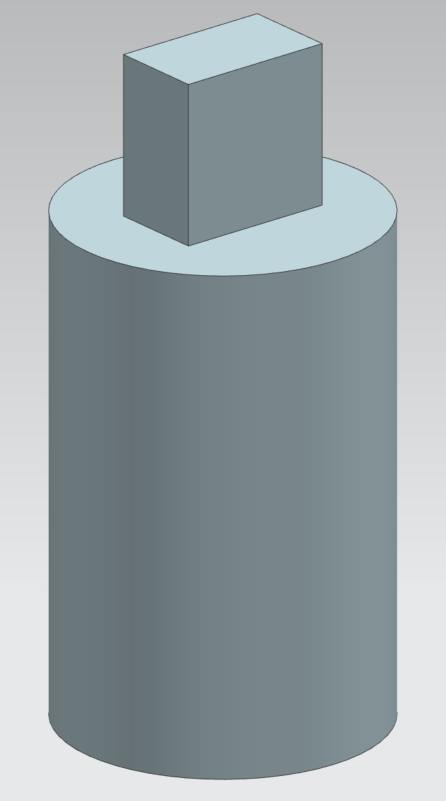
\includegraphics[width=\textwidth]{img/1.jpg}
    \caption{Shaft Adapter 3D}
  \end{minipage}
  \hfill
  \begin{minipage}[b]{0.4\textwidth}
    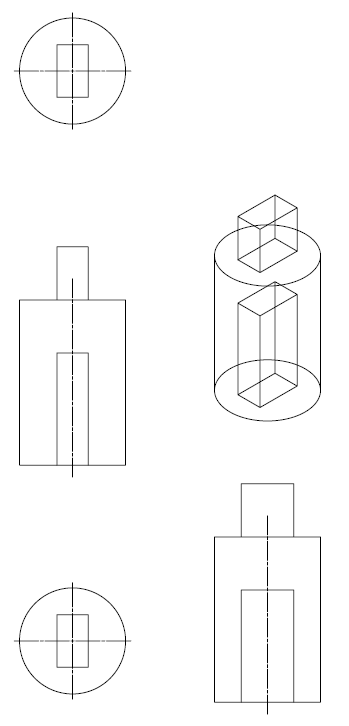
\includegraphics[width=\textwidth]{img/2.jpg}
    \caption{2D Engineering Drawing of Shaft Adapter}
  \end{minipage}
\end{figure}
\end{minipage}
\end{center}

\subsubsection*{Panning Control}
The functionality of the Automatic Panning will be to rotate the entire shooting mechanism or the shooting barrel about the z-axis so the mechanism is able to cover all of the shooting zones as specified in the requirements. \\ \\
The components designed for the panning stage include an acrylic base plate, a rapid prototyped worm wheel gear ring, the worm, and a motor bracket. The base plate clearance mounting holes were made using a workshop drill press / milling machine. The rapid prototyped stepper motor bracket is mounted to the base plate and adjusted so that correct gear engagement is achieved. The Lazy Susan bearing is positioned 10 mm above the plate using spacers and longer \#6?32 screws, washers, and nuts. The worm gear is designed as a ring shape to reduce rapid prototyping material consumption. A corresponding hole pattern mates to the top plate of the Lazy Susan bearing. The optical switch is used to home the system at power up and align the system in the direction required with a reference and from there on the system will always be aware of its position. Optical switches allow for high repeatability making it a very applicable sensor to use in the prototype. 

\begin{center}
\begin{minipage}[b]{0.8\textwidth}
\begin{figure}[H]
  \centering
  \begin{minipage}[b]{0.4\textwidth}
    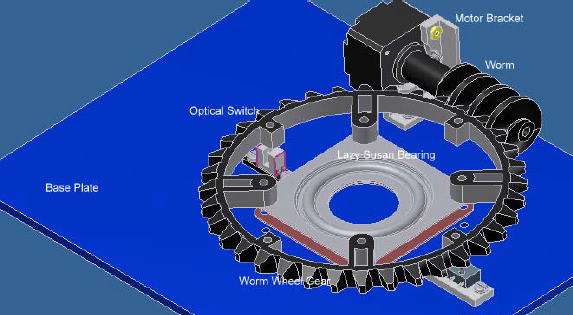
\includegraphics[width=\textwidth]{img/3.jpg}
    \caption{Base Design and Assembly}
  \end{minipage}
  \hfill
  \begin{minipage}[b]{0.4\textwidth}
    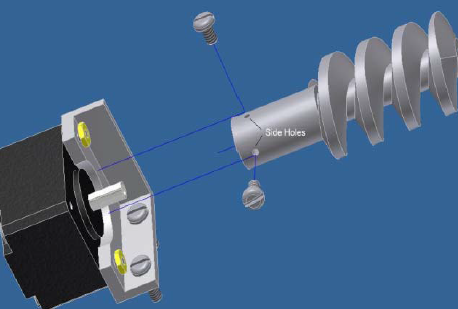
\includegraphics[width=\textwidth]{img/4.jpg}
    \caption{Worm Gear Coupler}
  \end{minipage}
\end{figure}
\end{minipage}
\end{center}

\begin{figure}[H]
   \centering
   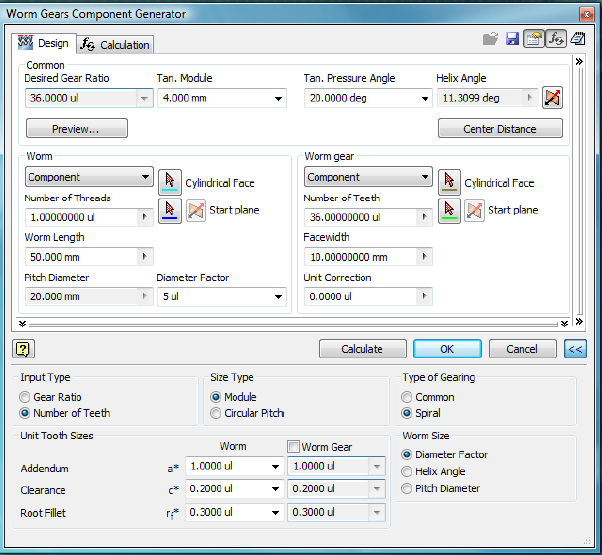
\includegraphics[width=0.6\textwidth]{img/5.jpg} % requires the graphicx package
   \caption{Azimuth Stage Autodesk Inventor Design Accelerator Worm Gear Parameters}
   \label{fig:hw5}
\end{figure}

\subsubsection*{Spinning Feeder Cutout}
The spinning feeder cutout is fixed to the shaft of the stepper motor inside the bucket to guide the table tennis balls into the \textit{Inner Tube}. The cutout is laser cut from a thin and sturdy sheet of wood so it has enough thickness (contact surface area) to easily push the table tennis balls around. There will be a lot of balls going in and out of the feeder cutout continuously so it has the sharp edges to hold the ball in once its captured and 45mm diameter semi circles to easily allow the 40mm table tennis balls to slide into the pockets.  

\begin{figure}[H]
   \centering
   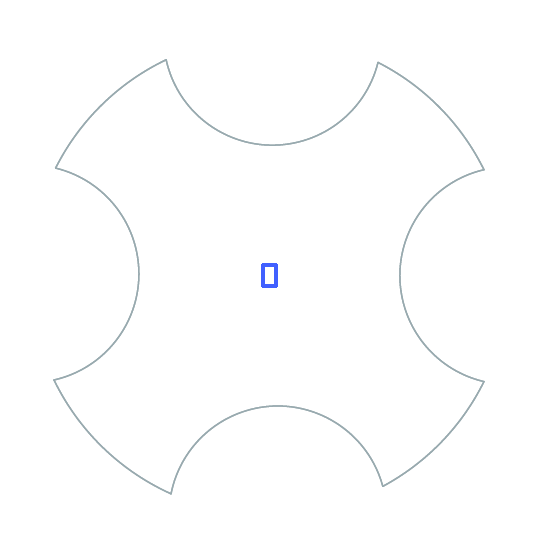
\includegraphics[width=0.3\textwidth]{img/6.jpg} % requires the graphicx package
   \caption{Feeder Cutout from topview for laser cutting  }
   \label{fig:hw6}
\end{figure}

\subsubsection*{Inner Tube}
The inner tube is designed to hold table tennis balls to be shot out by the shooting mechanism, as well as have solid support hold the shooting mechanism pipe structure. The diameter of the inner tube is 45mm to allow the ball to be easily fed into the tube but restrict jittering when traveling through the pipe.

\begin{figure}[H]
   \centering
   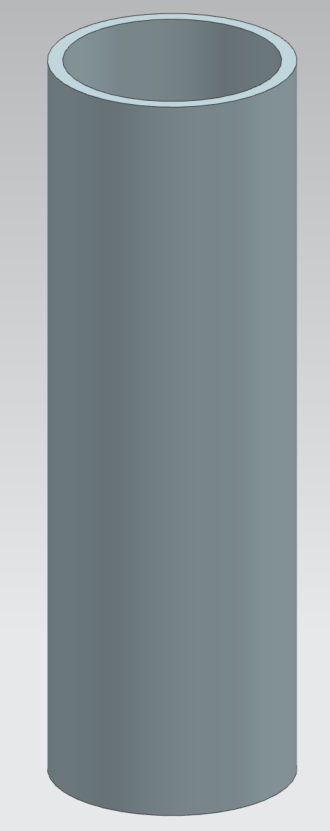
\includegraphics[width=0.2\textwidth]{img/7.jpg} % requires the graphicx package
   \caption{CAD design of a Inner Tube }
   \label{fig:hw7}
\end{figure}

 
\subsubsection*{Motor Bracket and Outer Tube}
A custom designed motor bracket is used to mount the DC motor onto the outer PVC tube to create our preliminary shooting mechanism. The motor has a cylindrical housing thus making it difficult to fix onto anything especially onto another cylindrical object, the Outer Tube. The motor has to be mounted securely and tightly to minimize the vibrations into the shooting mechanism which could translate onto the entire system.  

\begin{center}
\begin{minipage}[b]{1.0\textwidth}
\begin{figure}[H]
  \centering
  \begin{minipage}[b]{0.2\textwidth}
    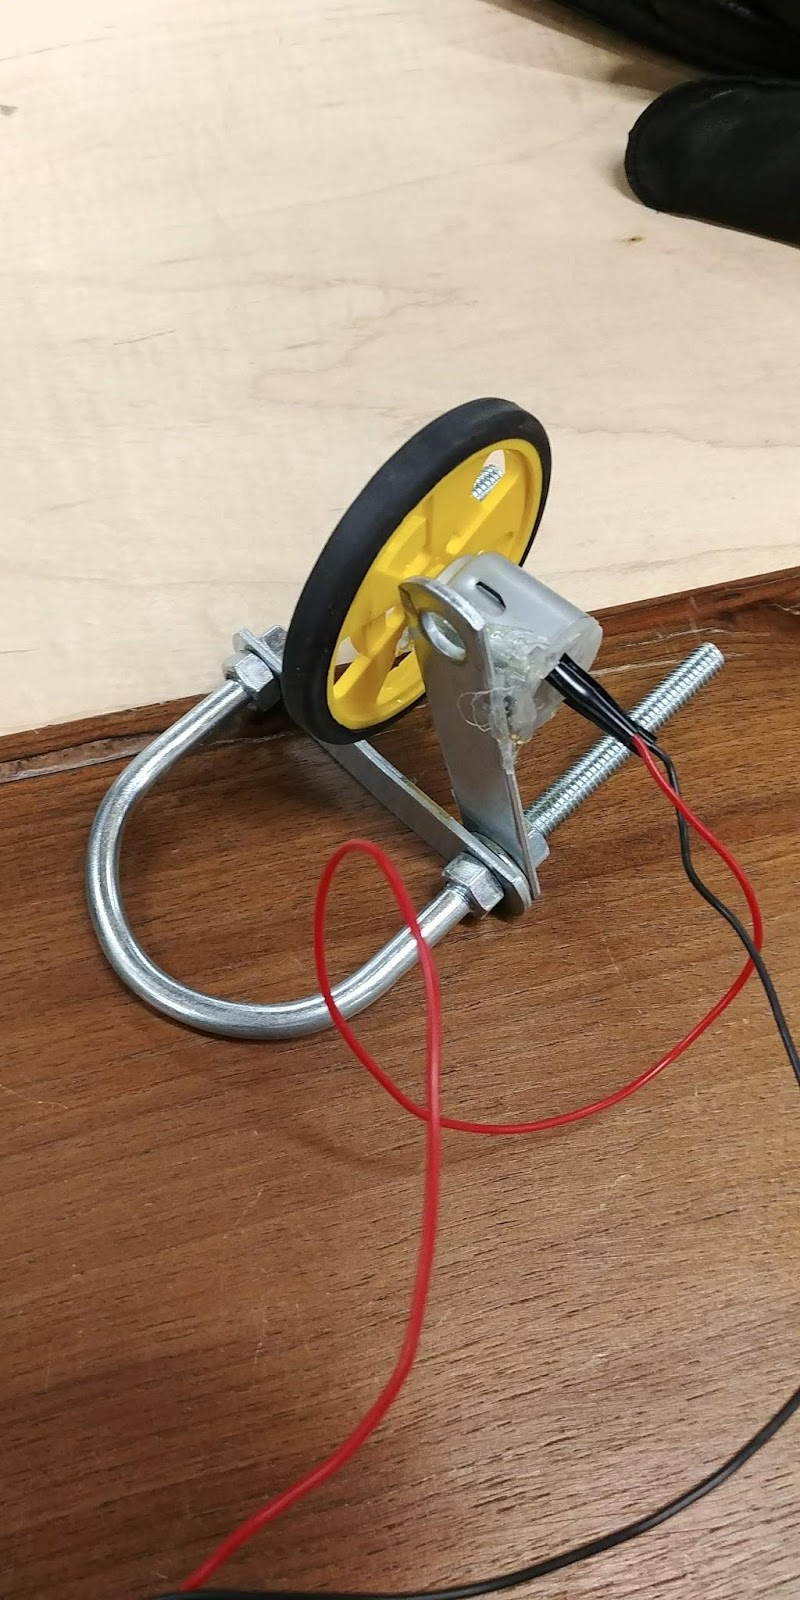
\includegraphics[width=\textwidth]{img/8.jpg}
    \caption{Motor Bracket}
  \end{minipage}
  \hfill
  \begin{minipage}[b]{0.2\textwidth}
    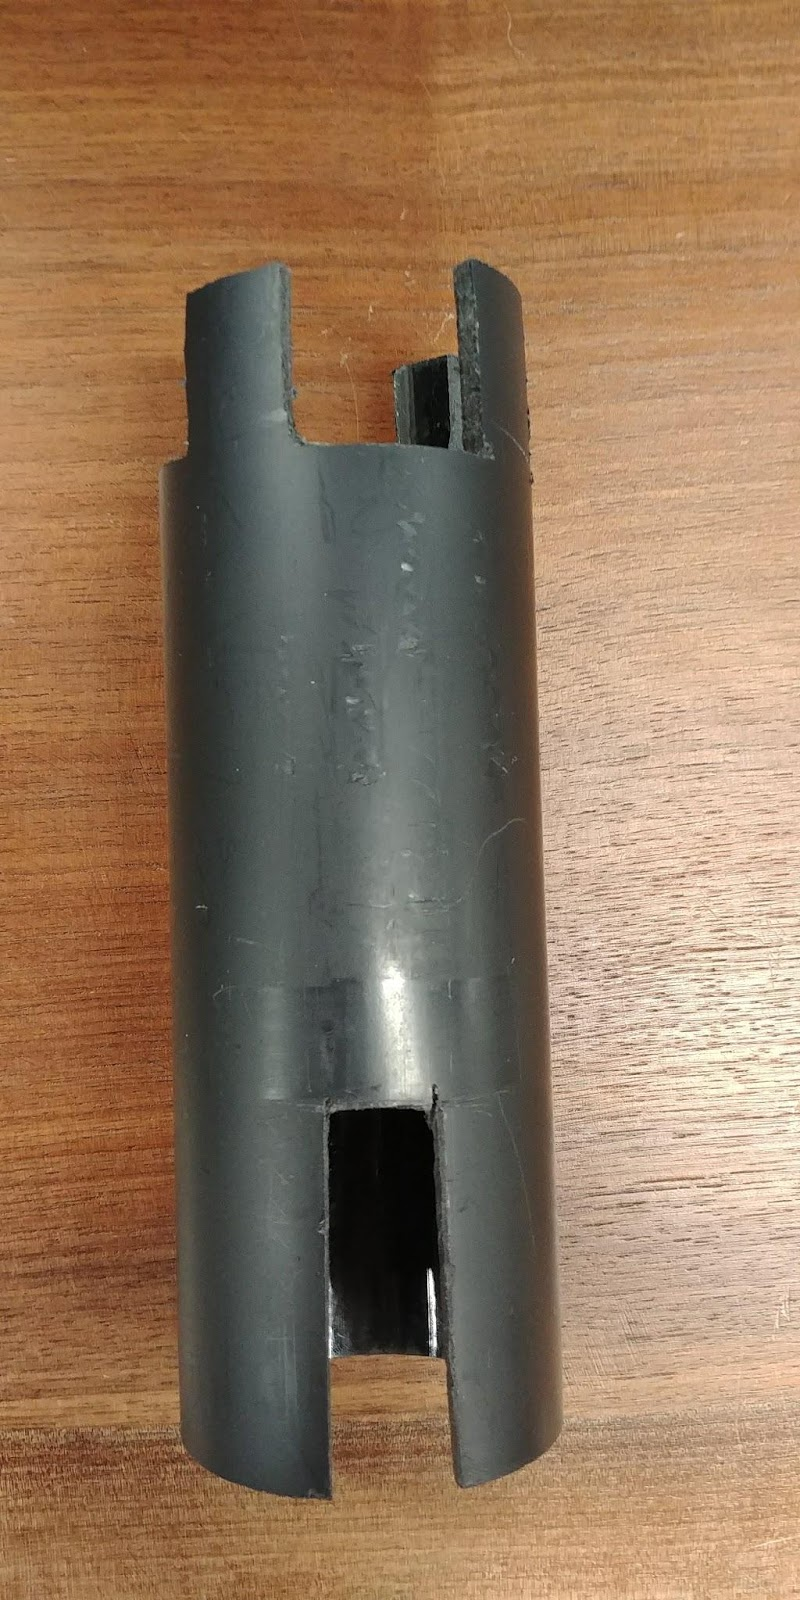
\includegraphics[width=\textwidth]{img/9.jpg}
    \caption{Outer Tube }
  \end{minipage}
  \hfill
  \begin{minipage}[b]{0.2\textwidth}
    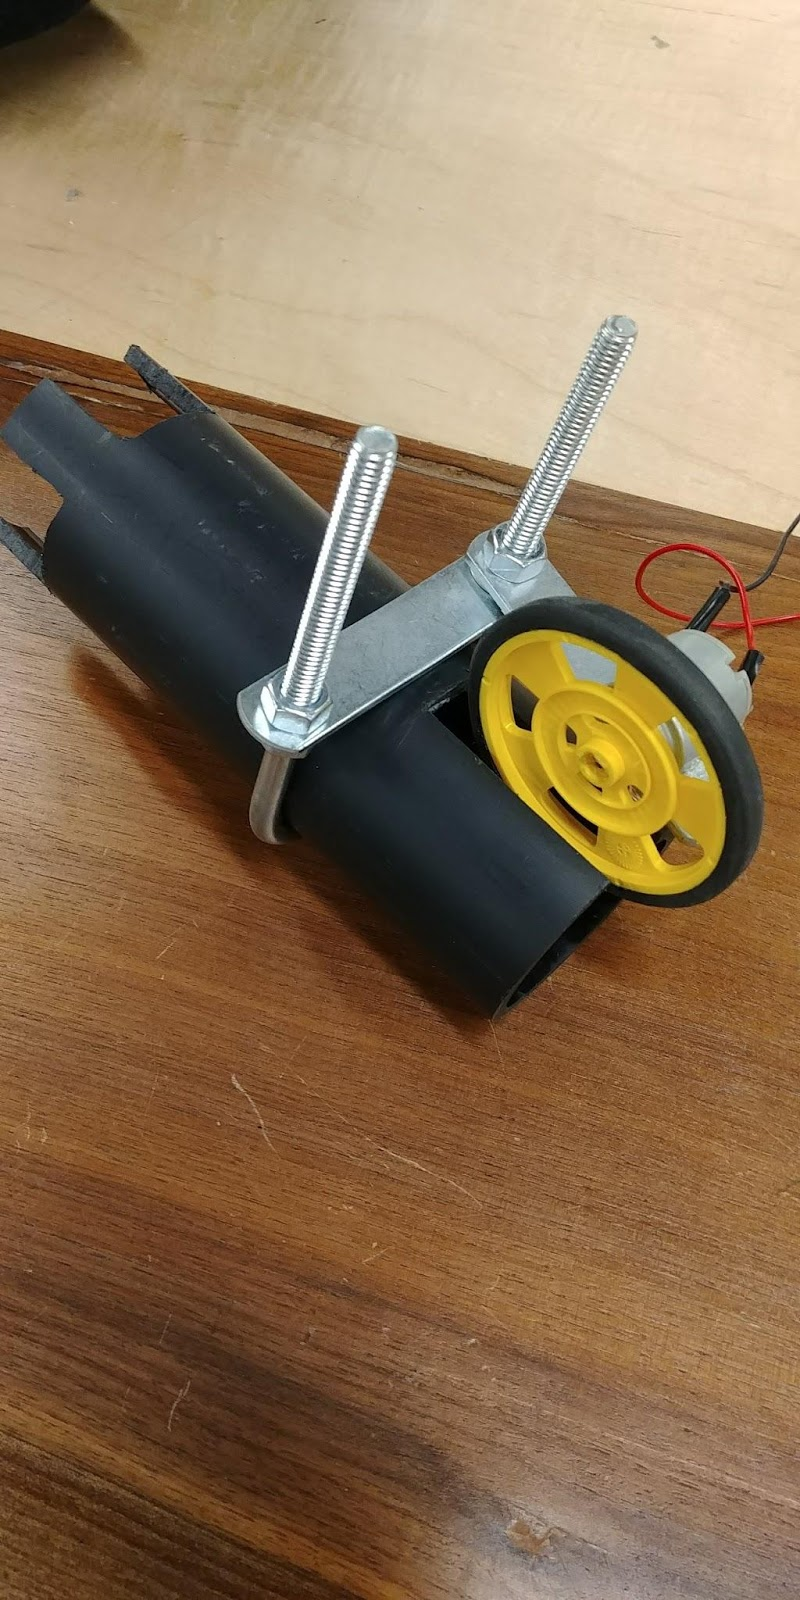
\includegraphics[width=\textwidth]{img/10.jpg}
    \caption{Motor with Motor Bracket attached to the Outer Tube }
  \end{minipage}
\end{figure}
\end{minipage}
\end{center}

\subsubsection*{Roll Control}
The roll control part will act as a manual control for the user to decide the type of spin to give the table tennis ball for the current session. The roll control part acts as the male end of a locking mechanism, which will fix the shooter in either a 0, 90, 180, or 270 degree angle. With the roll control settings, the user will be able to manually change the roll setting to experience a topspin, backspin, and left or right spin.The roll control part will be fixed on the base end of the inner shaft of the shooter. The outer shaft of the shooter will then be able to lock into the desired position.

\begin{center}
\begin{minipage}[b]{0.8\textwidth}
\begin{figure}[H]
  \centering
  \begin{minipage}[b]{0.4\textwidth}
    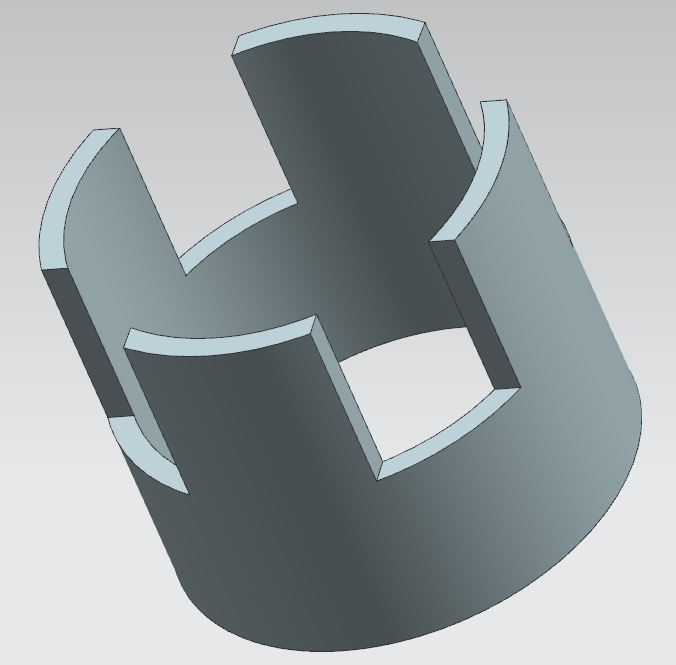
\includegraphics[width=\textwidth]{img/11.jpg}
    \caption{CAD design for Roll Control component }
  \end{minipage}
  \hfill
  \begin{minipage}[b]{0.4\textwidth}
    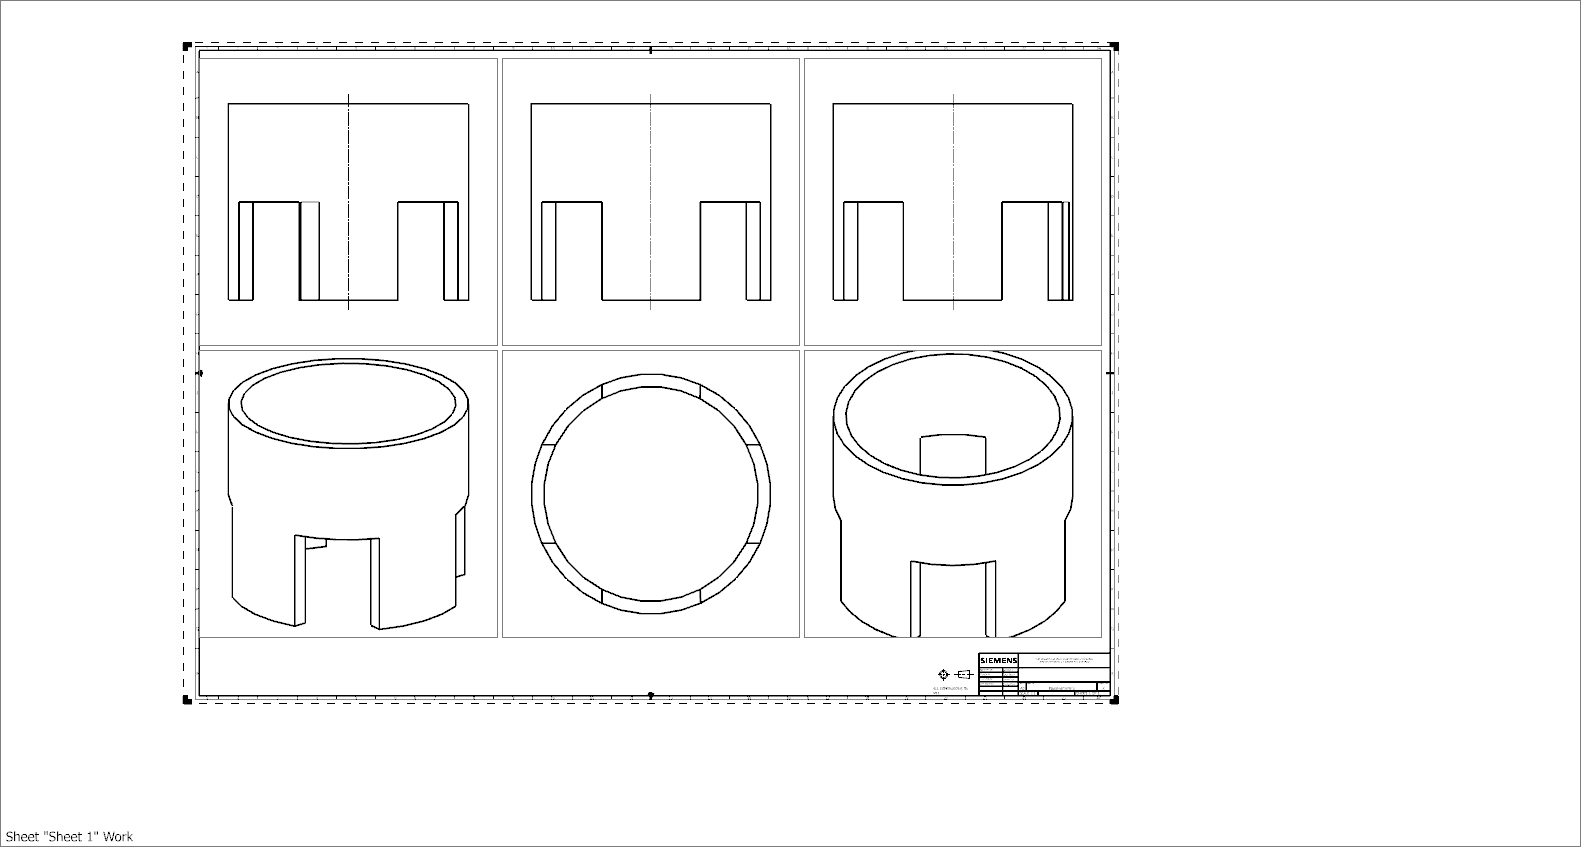
\includegraphics[width=\textwidth]{img/12.jpg}
    \caption{2D Engineering Drawing of Roll Control Component}
  \end{minipage}
\end{figure}
\end{minipage}
\end{center}

\subsubsection*{Base, Support Brackets and Bucket}
The base is made out of a hardwood and laser cut to an appropriate size. The base acts as a fixture to attach the bucket supports to the azimuth stage. There are two metal support brackets which are made out of stainless steel, and lift the bucket to an appropriate height above the base. The bottom of the supports are screwed into the hardwood base, and the top of the supports are bolted to the bucket. The bucket is 8in x 7in and is large enough to hold at least 20 balls without overfilling.

\begin{center}
\begin{minipage}[b]{0.8\textwidth}
\begin{figure}[H]
  \centering
  \begin{minipage}[b]{0.4\textwidth}
    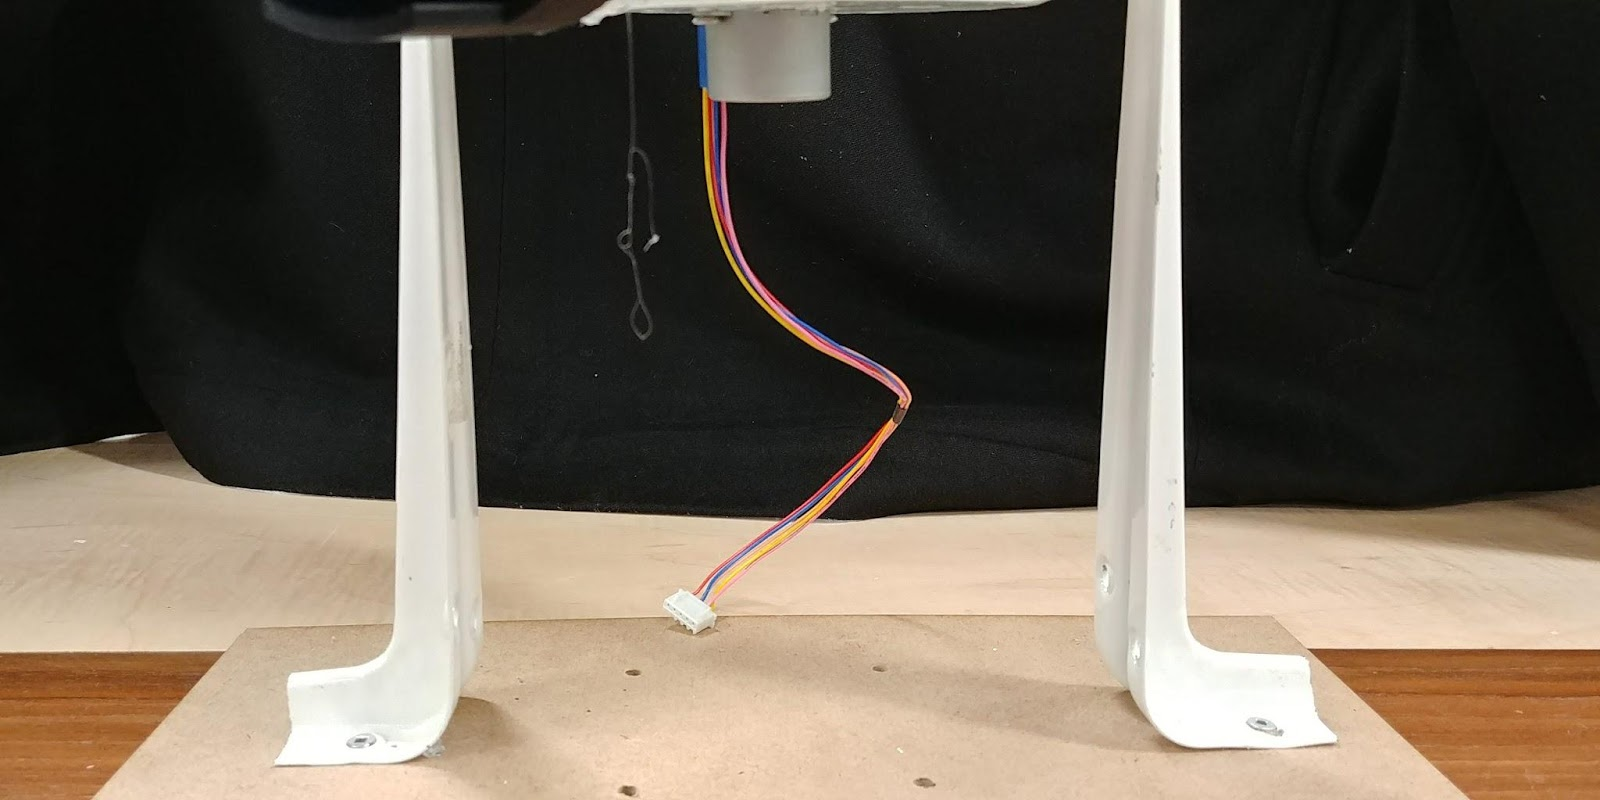
\includegraphics[width=\textwidth]{img/13.jpg}
    \caption{Base with Support Brackets attached }
  \end{minipage}
  \hfill
  \begin{minipage}[b]{0.4\textwidth}
    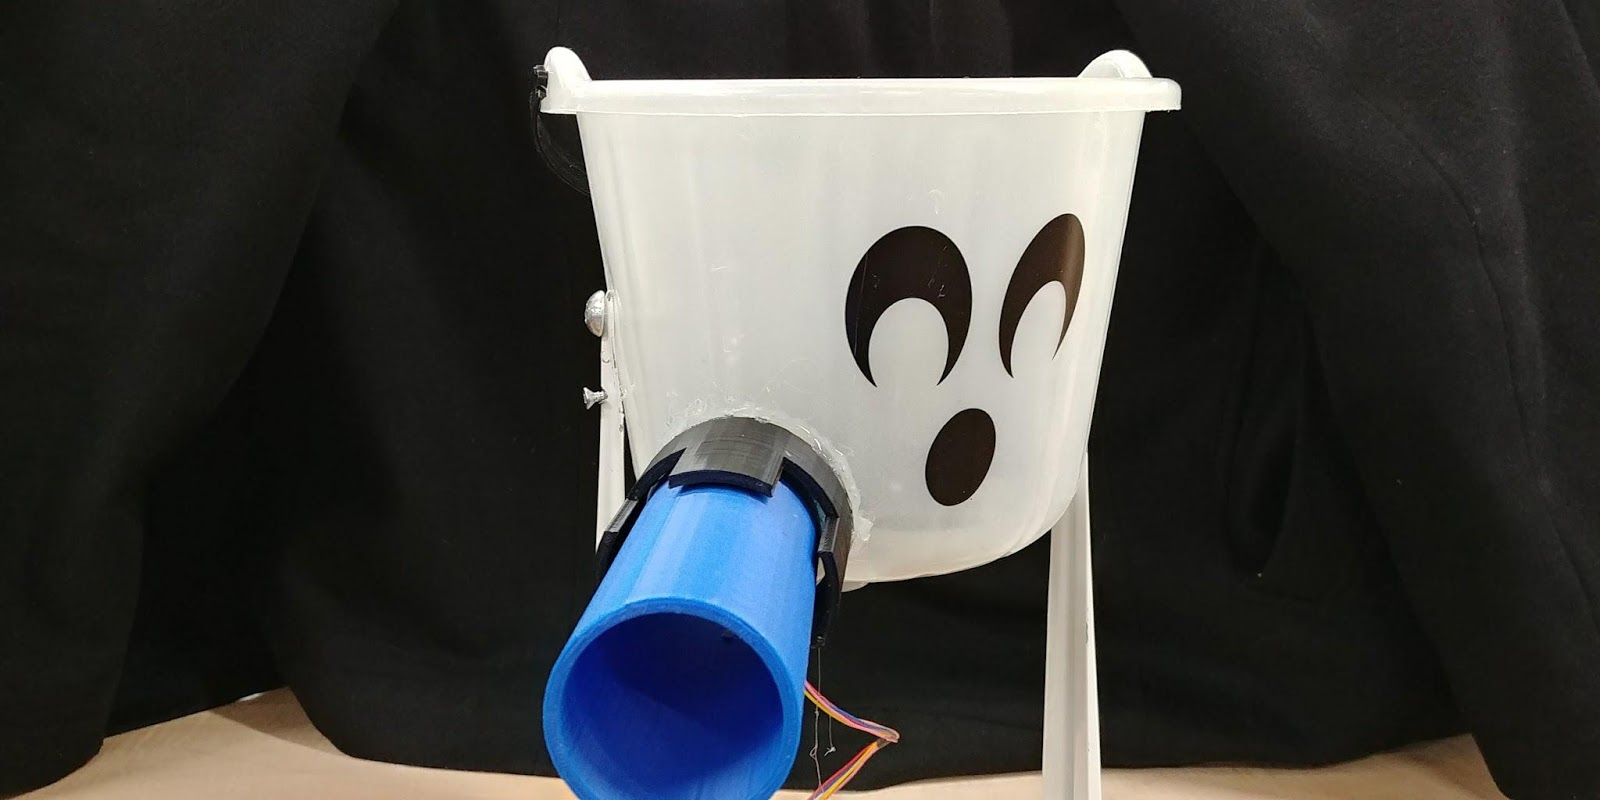
\includegraphics[width=\textwidth]{img/14.jpg}
    \caption{Bucket with Inner Tune and Roll Control attached }
  \end{minipage}
\end{figure}
\end{minipage}
\end{center}

\subsubsection*{Pitch Control}
The pitch control consists of a screw that pierces through the support beam and bucket, to hold the shooter at a certain angle. The range of angles are as followed: -15�,0�,15�,30�,45�, and are set by pre drilled holes in the bucket. This design needs to be optimized with a bolt in order to further secure the pitch and eliminate error.

\begin{center}
\begin{minipage}[b]{0.6\textwidth}
\begin{figure}[H]
  \centering
  \begin{minipage}[b]{0.4\textwidth}
    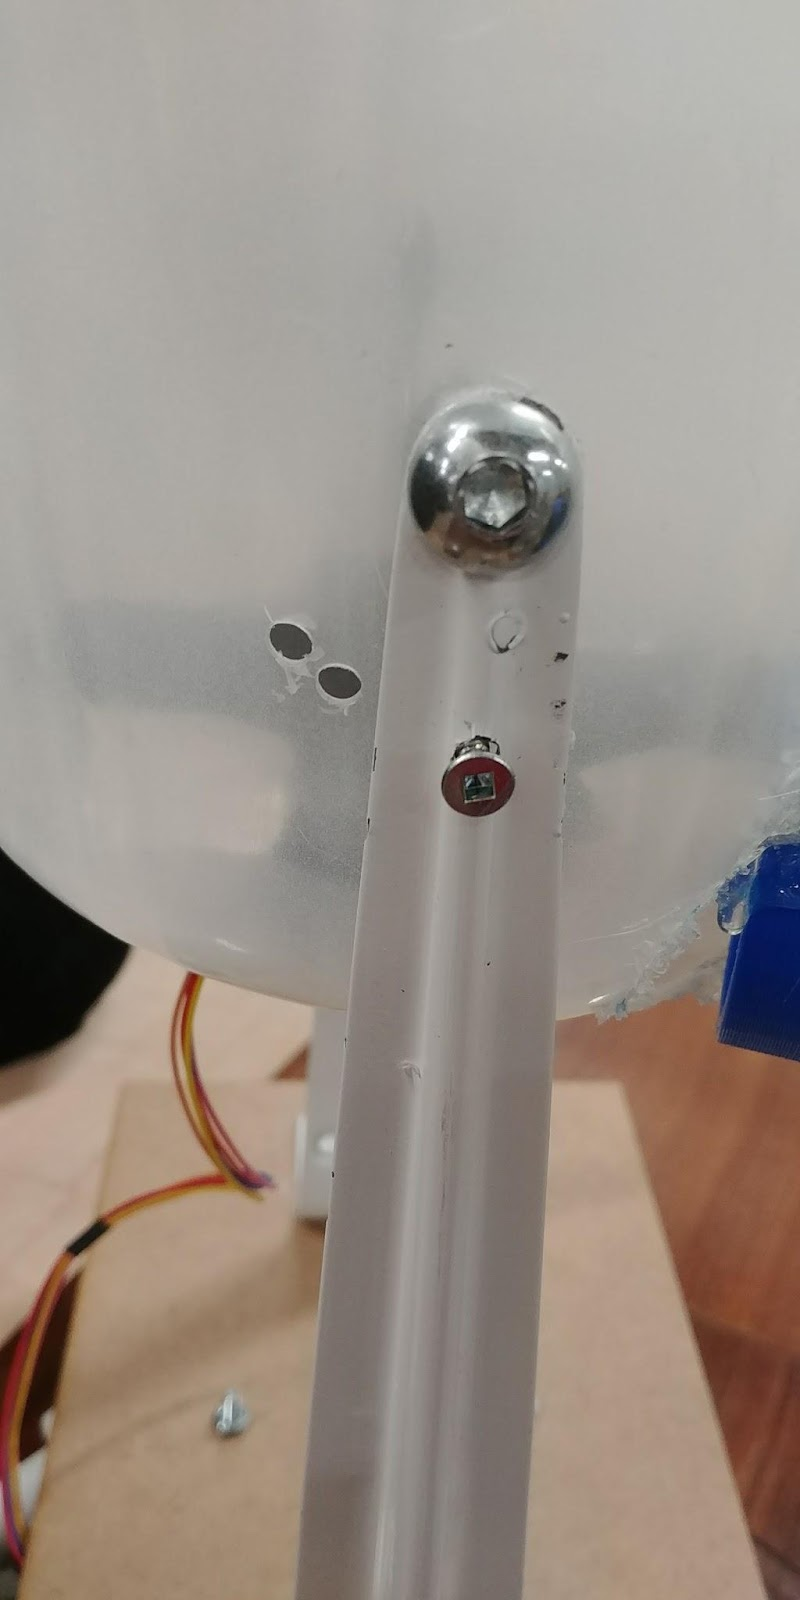
\includegraphics[width=\textwidth]{img/15.jpg}
    \caption{Pitch Control slots }
  \end{minipage}
  \hfill
  \begin{minipage}[b]{0.4\textwidth}
    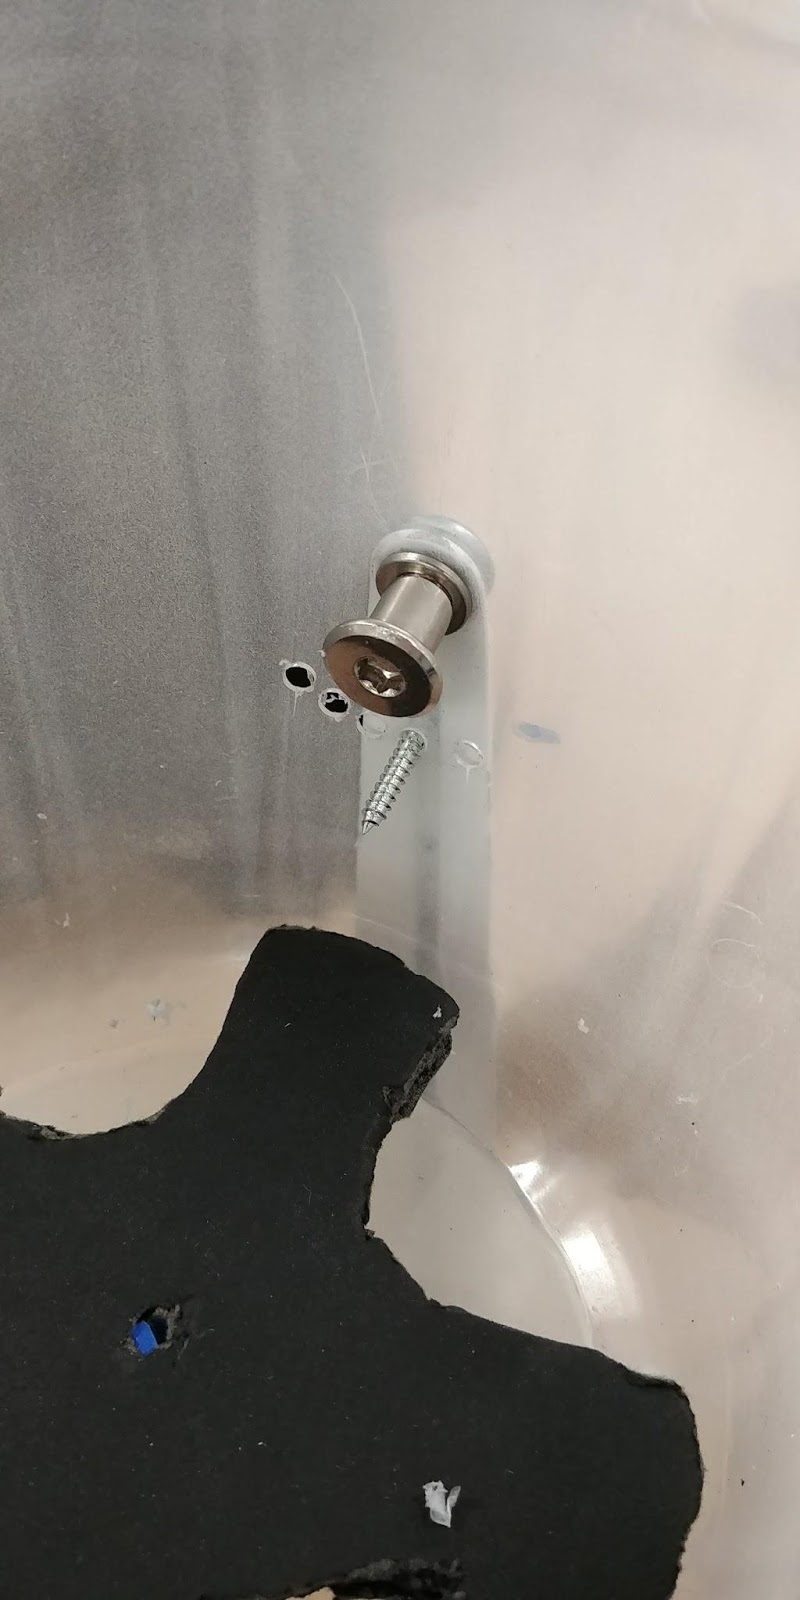
\includegraphics[width=\textwidth]{img/16.jpg}
    \caption{Pitch Control Holding Pin from Inside }
  \end{minipage}
\end{figure}
\end{minipage}
\end{center}

\subsection{Electrical Components}
\subsubsection*{Stepper Motors}
We chose a Japan Servo KP35FM2-035 stepper motor for the panning assembly because of its torque and step accuracy. To make the panning smooth as possible the motor provides 200 steps per revolution (1.8 degrees per step) from this stepper is sufficient for our purposes. The max torque is 700 g/cm at 24 VDC / 500mA but due to microcontroller restrictions and we are only using a torque of approximately 250g/cm to operate at a around 9VDC. At this lower voltage the stepper motor combined with the worm gear train provides enough torque to move the system (panning) at a sufficient speed.
A gear stepper motor (model 28BYJ48) with a driver is utilized for the automatic feeding of the balls into shooting barrel functionality as the stepper motor would not require any position encoder as well as the stepper motor will have predictable movements. This motor generates 300 g/cm torque at a voltage of 5VDC. This motor will be continuously running during the operation of the system at varying speeds and a ball will enter the Inner Tube at every quarter turn of the Feeder Cutout. The stepper has 64 steps per revolution (5.625 degrees per step) so every 16 steps the stepper moves, a ball will be fed into the feeder. This low-step count motor is good for our purposes because it allows the stepper to function at higher RPMs than other higher step count similar frame size motors. 

\begin{center}
\begin{minipage}[b]{0.8\textwidth}
\begin{figure}[H]
  \centering
  \begin{minipage}[b]{0.4\textwidth}
    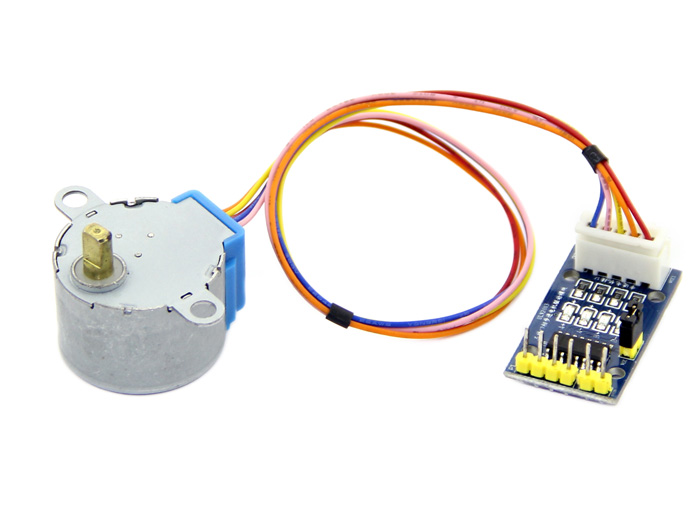
\includegraphics[width=\textwidth]{img/17.jpg}
    \caption{Gear Stepper Motor (Model 28BYJ48) with a Driver}
  \end{minipage}
  \hfill
  \begin{minipage}[b]{0.4\textwidth}
    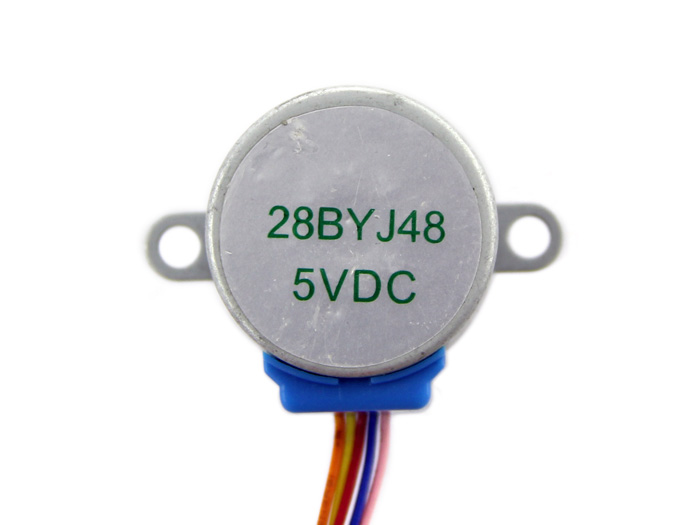
\includegraphics[width=\textwidth]{img/18.jpg}
    \caption{Stepper Motor 28BYJ48 Mounting Holes}
  \end{minipage}
\end{figure}
\end{minipage}
\end{center}

\subsubsection*{DC Motors}
For the ball shooter, a DC Motor purchased from Sayal Electronics and Hobbies is used as the system will require high speeds and high torques to shoot out ping pong balls. The DC motor operates between 3-6 volts, can reach a max RPM of 17,000, has a 2mm shaft diameter and max torque of 20.72 g/cm. Although the table tennis balls don't account for much weight the motor torque needs to be sufficient enough so that the wheel attached to the shaft can push on the ball, make contact and toss it out as required speeds. The DC Motor will be controlled using the PWM method for speed control.

\begin{center}
\begin{minipage}[b]{0.6\textwidth}
\begin{figure}[H]
  \centering
  \begin{minipage}[b]{0.4\textwidth}
    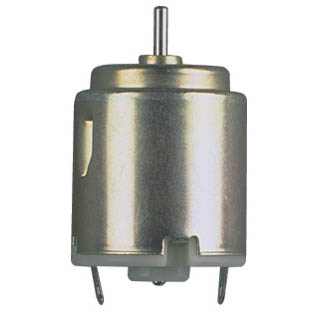
\includegraphics[width=\textwidth]{img/19.jpg}
    \caption{MOTOR DC 3-6VOLTS 17000RPM 2MM SHAFT 20.72G/CM TORQUE}
  \end{minipage}
  \hfill
  \begin{minipage}[b]{0.4\textwidth}
    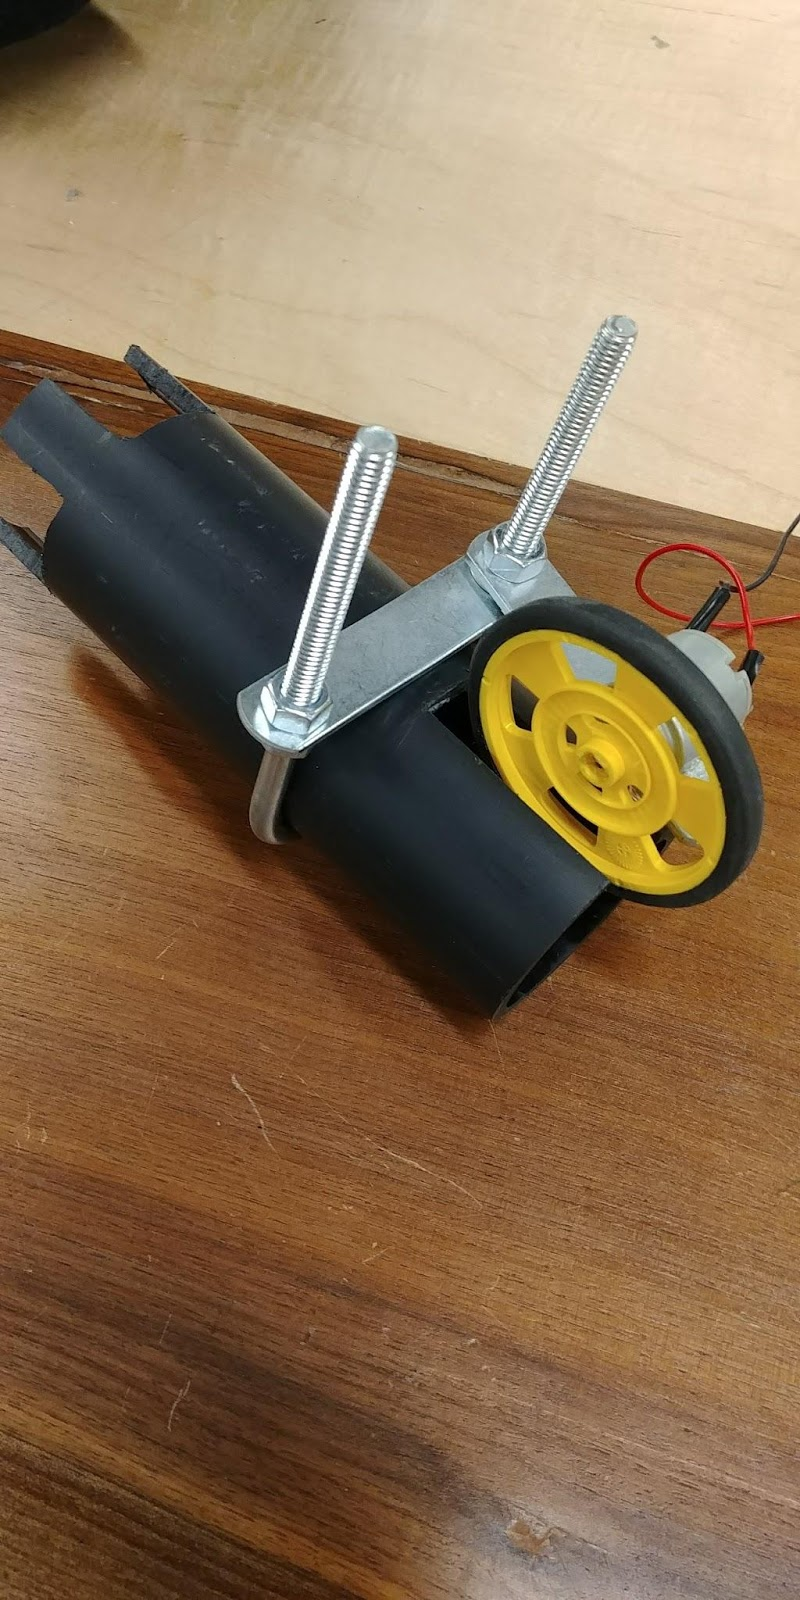
\includegraphics[width=\textwidth]{img/20.jpg}
    \caption{DC Motor attached to the Motor Bracket onto the Outer Tube}
  \end{minipage}
\end{figure}
\end{minipage}
\end{center}

\subsubsection*{Arduino}
Arduino UNO microcontroller is used to control all of the IPO (Input Process Output) processes between the sensors, actuators and Smart Serve. Arduino is chosen because it has a hardware platform setup and allows programming and serial communication over USB so designing so a PCB is not necessary. It is fast for our purposes, there is a lot of libraries available to use and lots of hardware modules designed for Arduino UNO. Also, this microcontroller easily interfaces with the hardware used in this prototype. 

\section{Module-Requirement Traceability Matrix}
\begin{table}[H]
\centering
\caption{Module-Functional Requirement Traceability Matrix}
\label{my-label}
\begin{tabular}{|l|l|l|l|l|l|l|l|}
\hline
Requirement ID & SS & SR & SM & CV & DS & SMech & UI \\ \hline
F1             &    &    & X  &    &    & X     &    \\ \hline
F2             &    &    &    &    &    & X     &    \\ \hline
F3             &    &    &    &    &    & X     &    \\ \hline
F4             &    &    &    &    &    & X     &    \\ \hline
F5             &    &    &    & X  &    &       &    \\ \hline
F6             &    &    &    &    & X  &       &    \\ \hline
F7             &    &    &    &    & X  &       &    \\ \hline
F8             &    &    &    &    & X  &       &    \\ \hline
F9             &    &    &    &    & X  &       &    \\ \hline
F10            & X  &    &    &    &    &       & X  \\ \hline
F11            & X  &    &    &    &    &       & X  \\ \hline
F12            & X  &    &    &    &    &       & X  \\ \hline
F13            &    &    &    &    & X  &       & X  \\ \hline
F14            &    & X  &    &    &    &       &    \\ \hline
F15            &    & X  &    &    &    &       &    \\ \hline
F16            & X  &    &    &    & X  &       & X  \\ \hline
F17            & X  &    &    &    & X  &       & X  \\ \hline
F18            & X  &    &    &    &    &       &    \\ \hline
\end{tabular}
\end{table}

\begin{table}[H]
\centering
\caption{Module Non-Functional Requirement Traceability Matrix}
\label{my-label}
\begin{tabular}{|l|l|l|l|l|l|l|l|}
\hline
Requirement ID & SS & SR & SM & CV & DS & SMech & UI \\ \hline
LF1            &    &    &    &    &    &       & X  \\ \hline
UH1            &    &    &    &    &    &       & X  \\ \hline
UH2            &    &    &    &    &    &       & X  \\ \hline
P1             &    &    &    &    &    &       & X  \\ \hline
P2             & X  &    &    &    & X  &       &    \\ \hline
P4             &    &    &    &    & X  &       &    \\ \hline
P5             & X  &    &    &    &    &       &    \\ \hline
OE2            &    &    &    & X  &    &       &    \\ \hline
MS2            & X  &    &    &    & X  &       & X  \\ \hline
S1             &    &    &    &    & X  &       &    \\ \hline
S2             &    &    &    &    & X  &       &    \\ \hline
P1             & X  &    &    &    & X  &       &    \\ \hline
LC1            &    &    &    &    &    &       &    \\ \hline
HS1            &    &    & X  &    &    & X     &    \\ \hline
HS2            &    &    &    &    &    & X     &    \\ \hline
HS3            &    &    &    &    &    & X     &    \\ \hline
HS4            &    &    &    &    &    & X     &    \\ \hline
HS5            &    &    &    &    &    & X     &    \\ \hline
\end{tabular}
\end{table}
\newpage
\section{Appendix}

\begin{sidewaysfigure}[ht]
   \centering
   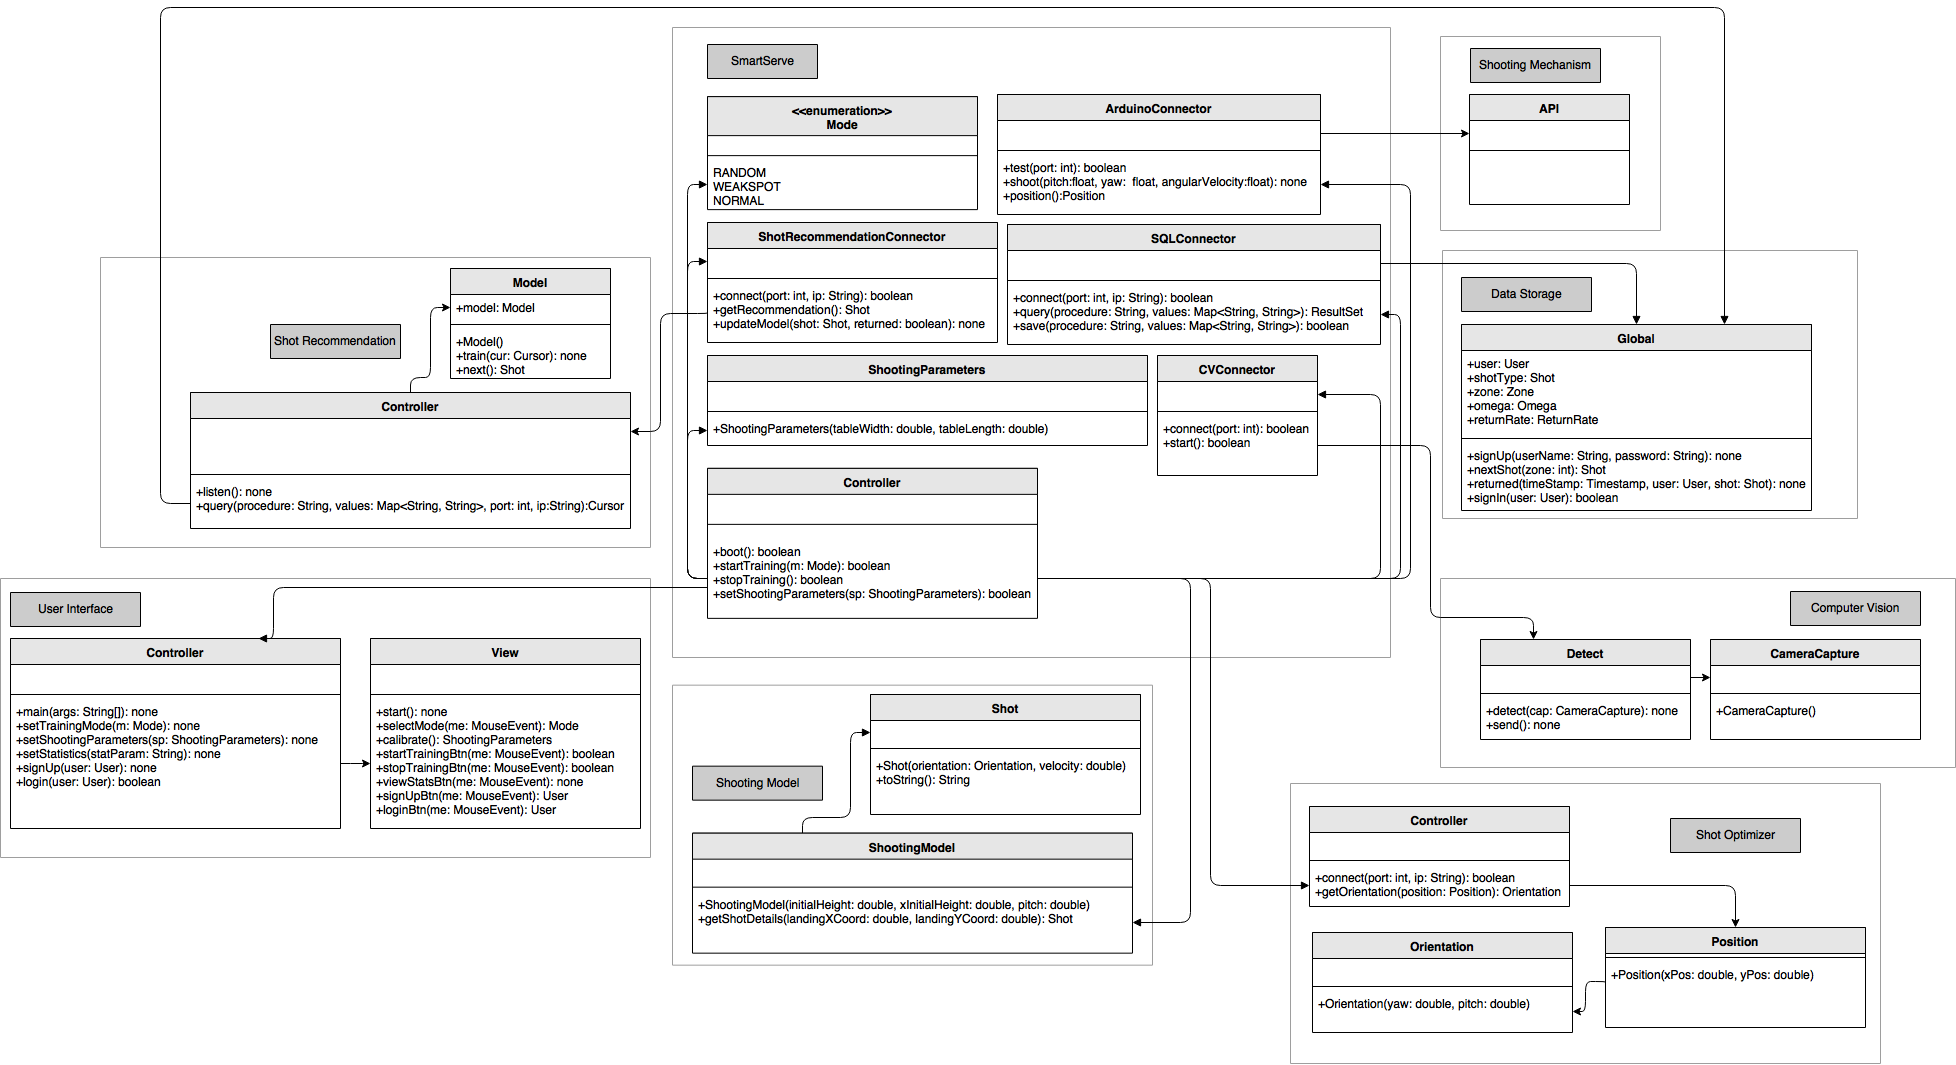
\includegraphics[width=\textwidth]{diagram/DCD.png} % requires the graphicx package
   \caption{Detailed Class Diagram}
   \label{fig:dcd}
\end{sidewaysfigure}

\end{document}
